%%%%%%%%%%%%%%%%%%%%%%%%%%%%%%%%%%%%%%%%%
% Masters/Doctoral Thesis 
% LaTeX Template
% Version 1.43 (17/5/14)
%
% This template has been downloaded from:
% http://www.LaTeXTemplates.com
%
% Original authors:
% Steven Gunn 
% http://users.ecs.soton.ac.uk/srg/softwaretools/document/templates/
% and
% Sunil Patel
% http://www.sunilpatel.co.uk/thesis-template/
%
% License:
% CC BY-NC-SA 3.0 (http://creativecommons.org/licenses/by-nc-sa/3.0/)
%
% Note:
% Make sure to edit document variables in the Thesis.cls file
%
%%%%%%%%%%%%%%%%%%%%%%%%%%%%%%%%%%%%%%%%%

%----------------------------------------------------------------------------------------
%	PACKAGES AND OTHER DOCUMENT CONFIGURATIONS
%----------------------------------------------------------------------------------------

\documentclass[12pt, oneside]{Thesis} % The default font size and one-sided printing (no margin offsets)

\graphicspath{{Pictures/}} % Specifies the directory where pictures are stored
\usepackage{cite}
\usepackage{graphicx}
\usepackage[square, numbers, comma, sort&compress]{natbib}
\usepackage{listings}
\usepackage{color} 
\usepackage{amsmath}
\usepackage{algorithm}
\usepackage[noend]{algpseudocode}
\makeatletter
\def\BState{\State\hskip-\ALG@thistlm}
\makeatother

% Use the natbib reference package - read up on this to edit the reference style; if you want text (e.g. Smith et al., 2012) for the in-text references (instead of numbers), remove 'numbers' 
\hypersetup{urlcolor=blue, colorlinks=true} % Colors hyperlinks in blue - change to black if annoying
\title{\ttitle} % Defines the thesis title - don't touch this
\definecolor{gray}{rgb}{0.4,0.4,0.4}
\definecolor{darkblue}{rgb}{0.0,0.0,0.6}
\definecolor{cyan}{rgb}{0.0,0.6,0.6}

\lstset{
	basicstyle=\ttfamily,
	columns=fullflexible,
	showstringspaces=false,
	commentstyle=\color{gray}\upshape
}

\lstdefinelanguage{XML}
{
	morestring=[b]",
	morestring=[s]{>}{<},
	morecomment=[s]{<?}{?>},
	stringstyle=\color{black},
	identifierstyle=\color{darkblue},
	keywordstyle=\color{cyan},
	morekeywords={xmlns,version,type}% list your attributes here
}

\definecolor{dkgreen}{rgb}{0,0.6,0}
\definecolor{gray}{rgb}{0.5,0.5,0.5}
\definecolor{mauve}{rgb}{0.58,0,0.82}

\lstset{frame=tb,
	language=Java,
	aboveskip=3mm,
	belowskip=3mm,
	showstringspaces=false,
	columns=flexible,
	basicstyle={\small\ttfamily},
	numbers=none,
	numberstyle=\tiny\color{gray},
	keywordstyle=\color{blue},
	commentstyle=\color{dkgreen},
	stringstyle=\color{mauve},
	breaklines=true,
	breakatwhitespace=true
	tabsize=2
}

\begin{document}

\frontmatter % Use roman page numbering style (i, ii, iii, iv...) for the pre-content pages

\setstretch{1.3} % Line spacing of 1.3

% Define the page headers using the FancyHdr package and set up for one-sided printing
\fancyhead{} % Clears all page headers and footers
\rhead{\thepage} % Sets the right side header to show the page number
\lhead{} % Clears the left side page header

\pagestyle{fancy} % Finally, use the "fancy" page style to implement the FancyHdr headers

\newcommand{\HRule}{\rule{\linewidth}{0.5mm}} % New command to make the lines in the title page

% PDF meta-data
\hypersetup{pdftitle={\ttitle}}
\hypersetup{pdfsubject=\subjectname}
\hypersetup{pdfauthor=\authornames}
\hypersetup{pdfkeywords=\keywordnames}

%----------------------------------------------------------------------------------------
%	TITLE PAGE
%----------------------------------------------------------------------------------------

\begin{titlepage}
\begin{center}

\textsc{\LARGE \univname}\\[1.5cm] % University name
\textsc{\Large Doctoral Thesis}\\[0.5cm] % Thesis type

\HRule \\[0.4cm] % Horizontal line
{\huge \bfseries \ttitle}\\[0.4cm] % Thesis title
\HRule \\[1.5cm] % Horizontal line
 
\begin{minipage}{0.4\textwidth}
\begin{flushleft} \large
\emph{Author:}\\
\href{http://www.johnsmith.com}{\authornames} % Author name - remove the \href bracket to remove the link
\end{flushleft}
\end{minipage}
\begin{minipage}{0.4\textwidth}
\begin{flushright} \large
\emph{Supervisor:} \\
\href{http://www.jamessmith.com}{\supname} % Supervisor name - remove the \href bracket to remove the link  
\end{flushright}
\end{minipage}\\[3cm]
 
\large \textit{A thesi  submitted in fulfilment of the requirements\\ for the degree of \degreename}\\[0.3cm] % University requirement text
\textit{in the}\\[0.4cm]
\groupname\\\deptname\\[2cm] % Research group name and department name
 
{\large \today}\\[4cm] % Date
%\includegraphics{Logo} % University/department logo - uncomment to place it
 
\vfill
\end{center}

\end{titlepage}

%----------------------------------------------------------------------------------------
%	DECLARATION PAGE
%	Your institution may give you a different text to place here
%----------------------------------------------------------------------------------------
%
%\Declaration{
%
%\addtocontents{toc}{\vspace{1em}} % Add a gap in the Contents, for aesthetics
%
%I, \authornames, declare that this thesis titled, '\ttitle' and the work presented in it are my own. I confirm that:
%
%\begin{itemize} 
%\item[\tiny{$\blacksquare$}] This work was done wholly or mainly while in candidature for a research degree at this University.
%\item[\tiny{$\blacksquare$}] Where any part of this thesis has previously been submitted for a degree or any other qualification at this University or any other institution, this has been clearly stated.
%\item[\tiny{$\blacksquare$}] Where I have consulted the published work of others, this is always clearly attributed.
%\item[\tiny{$\blacksquare$}] Where I have quoted from the work of others, the source is always given. With the exception of such quotations, this thesis is entirely my own work.
%\item[\tiny{$\blacksquare$}] I have acknowledged all main sources of help.
%\item[\tiny{$\blacksquare$}] Where the thesis is based on work done by myself jointly with others, I have made clear exactly what was done by others and what I have contributed myself.\\
%\end{itemize}
% 
%Signed:\\
%\rule[1em]{25em}{0.5pt} % This prints a line for the signature
% 
%Date:\\
%\rule[1em]{25em}{0.5pt} % This prints a line to write the date
%}
%
%\clearpage % Start a new page

%----------------------------------------------------------------------------------------
%	QUOTATION PAGE
%----------------------------------------------------------------------------------------
%
%\pagestyle{empty} % No headers or footers for the following pages
%
%\null\vfill % Add some space to move the quote down the page a bit
%
%\textit{``Thanks to my solid academic training, today I can write hundreds of words on virtually any topic without possessing a shred of information, which is how I got a good job in journalism."}
%
%\begin{flushright}
%Dave Barry
%\end{flushright}
%
%\vfill\vfill\vfill\vfill\vfill\vfill\null % Add some space at the bottom to position the quote just right
%
%\clearpage % Start a new page
%
%%----------------------------------------------------------------------------------------
%%	ABSTRACT PAGE
%%----------------------------------------------------------------------------------------
%
%\addtotoc{Abstract} % Add the "Abstract" page entry to the Contents
%
%\abstract{\addtocontents{toc}{\vspace{1em}} % Add a gap in the Contents, for aesthetics
%
%The Thesis Abstract is written here (and usually kept to just this page). The page is kept centered vertically so can expand into the blank space above the title too\ldots
%}
%
%\clearpage % Start a new page
%
%%----------------------------------------------------------------------------------------
%%	ACKNOWLEDGEMENTS
%%----------------------------------------------------------------------------------------
%
%\setstretch{1.3} % Reset the line-spacing to 1.3 for body text (if it has changed)
%
%\acknowledgements{\addtocontents{toc}{\vspace{1em}} % Add a gap in the Contents, for aesthetics
%
%The acknowledgements and the people to thank go here, don't forget to include your project advisor\ldots
%}
%\clearpage % Start a new page
%
%%----------------------------------------------------------------------------------------
%%	LIST OF CONTENTS/FIGURES/TABLES PAGES
%%----------------------------------------------------------------------------------------

\pagestyle{fancy} % The page style headers have been "empty" all this time, now use the "fancy" headers as defined before to bring them back

\lhead{\emph{Contents}} % Set the left side page header to "Contents"
\tableofcontents % Write out the Table of Contents

\lhead{\emph{List of Figures}} % Set the left side page header to "List of Figures"
\listoffigures % Write out the List of Figures

\lhead{\emph{List of Tables}} % Set the left side page header to "List of Tables"
\listoftables % Write out the List of Tables
%
%%----------------------------------------------------------------------------------------
%%	ABBREVIATIONS
%%----------------------------------------------------------------------------------------
%
%\clearpage % Start a new page
%
%\setstretch{1.5} % Set the line spacing to 1.5, this makes the following tables easier to read
%
%\lhead{\emph{Abbreviations}} % Set the left side page header to "Abbreviations"
%\listofsymbols{ll} % Include a list of Abbreviations (a table of two columns)
%{
%\textbf{LAH} & \textbf{L}ist \textbf{A}bbreviations \textbf{H}ere \\
%%\textbf{Acronym} & \textbf{W}hat (it) \textbf{S}tands \textbf{F}or \\
%}
%
%
%%----------------------------------------------------------------------------------------
%%	DEDICATION
%%----------------------------------------------------------------------------------------
%
%\setstretch{1.3} % Return the line spacing back to 1.3
%
%\pagestyle{empty} % Page style needs to be empty for this page
%
%\dedicatory{For/Dedicated to/To my\ldots} % Dedication text
%
%\addtocontents{toc}{\vspace{2em}} % Add a gap in the Contents, for aesthetics

%----------------------------------------------------------------------------------------
%	THESIS CONTENT - CHAPTERS
%----------------------------------------------------------------------------------------

\mainmatter % Begin numeric (1,2,3...) page numbering

\pagestyle{fancy} % Return the page headers back to the "fancy" style

% Include the chapters of the thesis as separate files from the Chapters folder
% Uncomment the lines as you write the chapters

\chapter{Introduction} % Main chapter title

\label{Chapter 1} % For referencing the chapter elsewhere, use \ref{Chapter1} 

\lhead{Chapter 1 . \emph{Introduction}} % This is for the header on each page - perhaps a shortened title


Researchers in Artificial Intelligence (AI), and especially in the field of automated reasoning and problem resolving, are interested on the representation of the real world using logical models to define planning algorithms for these models. The "reasoning about actions and changes" field is one of the fields in  AI which focuses on problems involving world changes. In particular, since the 80s, planning algorithms were proposed so that, from an initial state, a goal state and a set of actions described as transitions between states, one can obtain a sequence of actions that leads from the initial state to the goal state.
\par Once the plan is built, it is executed by the controller of the simulated system. However, sometimes during the execution, the current state may not correspond to the expected state. Therefore, the controller can no longer proceed with the plan. This is called a {\em breakdown}.

These {\em breakdowns} can be caused by dynamic environment (external actions that modify the system state), or by an incomplete modeling of the real world. One common assumption is that the planner needs, in order to build a consistent plan, a complete and a faithful representation of the problem actions, called the \emph{knowledge domain}. 
Nevertheless, modeling such a complete domain requires significant knowledge-engineering effort, and even reveals to be impossible  \cite{gil1992acquiring}. For example, representing completely  the human activity in housing for the intelligent management of energy \cite{hurauxmodele} using logics is not realistic. The most challenging part in  modeling such a complex knowledge domain is to define the granularity with which we can construct a model  representing  accurately  the real world. This  implies representing each  action and the used devices taking into account the variability of the environment. 
%Thus, the existing models represent the general view of the world.
  In the real life, we frequently observe a combination of these two phenomena: an incomplete model and a dynamic environment. Therefore, it is necessary to define plan repair in order to face possible breakdowns. 
\par The goal of this master thesis is to propose a planning system that can recover from breakdowns taking into account the incompleteness of the model. Unlike the existing systems which suppose that 1) the model is  complete enough to be consistently fixed and  2) breakdowns are only caused by the dynamic nature of the environment, we consider breakdowns caused by incomplete knowledge domain and propose an algorithm . 
\par The outline of this report is as follow. We will first present  existing works in this domain: chapter 2 presents classical planning methods (from linear planning to hierarchical planning and  reactive approaches) and discussing their limits; chapter 3, present existing plan repair systems. In chapter 4, we propose Discolog, a hybrid system that combines the execution of a reactive HTN (Disco) with simple linear planning  to recover from breakdowns.  Chapter 5 presents the  implementation of this model and chapter 6  presents the experiments and validation of the proposed solution . We conclude this thesis by presenting ongoing and future work. 
%%What is dominance in social psychology
%Nonverbal Behavior and the Vertical Dimension of Social Relations: A Meta-Analysis
%
%\textbf{several representation of dominance :} 
%For example, dominance can be defined as a personality trait involving the motive to control others, the self-
%perception of oneself as controlling others, and/or as a behavioral
%outcome (success in controlling others or their resources). Status,
%involving an ascribed or achieved quality implying respect and
%privilege, does not necessarily include the ability to control others
%or their resources.
%
% Similarly, power defined as the capacity or
%structurally sanctioned right to control others or their resources
%does not necessarily imply prestige or respect. Other distinctions
%have also been drawn, including different functional bases of
%power, such as reward power, expert power, referent power, or
%coercive power (French and Raven, 1959), and outcome dependency
%(Stevens  Fiske, 2000). Some writers conceptualize dominance
%in terms of social skill (e.g., Burgoon  Dunbar, 2000; Byrne,
%2001). Some writers define dominance as the enactment of certain
%nonverbal or verbal behaviors (Rosa  Mazur, 1979). Authors do
%not use the various verticality terms such as power, dominance,
%and status in consistent ways, and often the terms are used without
%a clear definition.
%
%\textbf{Burgoon and dunber 2010}
%

%
%
%La dominance, d'un autre côté, se réfère à des comportements interactionnels dépendant du contexte et de la relation, dans lesquels le pouvoir est rendu saillant et l'influence est atteinte %(Burgoon et al., 1998; Mack, 1974; Rogers-Millar & Millar, 1979)
%dans le contexte de l'échange interpersonnel, la dominance est basée sur une combinaison de tempérament individuel et de caractéristiques situationnelles qui encouragent un comportement dominant. 
%Le dominance interpersonnelle est un comportement de communication basé sur la relation qui dépend du contexte et des motivations des individus impliqués
%
 
%Comme l'ont noté Emerson (1962) et d'autres théoriciens, le pouvoir équivaut à dépendre des autres et suppose donc une relation sociale.
%
%\textbf{Dyadic power theory:}
%
%
%Elle se base sur les échanges sociaux de pouvoir sur 4 éléments
%
%\begin{enumerate}
%	\item cette définition s'étend pour prendre en compte les échanges sociaux qui inclut les stratégies de communications qui deviennent manifestes durant l'interaction
%	\item Contrôle relationnel : elle reconnaît que l'autorité d'utiliser ou d'échanger des ressources dans les interactions est souvent accordée aux individus par les normes sociétales ainsi que par l'histoire relationnelle propre aux individus impliqués dans l'interaction.
%	
%	\item Cette représentation insiste sur l'idée que le pouvoir doit être vu relativement, ou par rapport aux autres. Ainsi, il reconnaît que le pouvoir est une construction dynamique et multidimensionnelle qui incorpore les perspectives des deux individus dans l'interaction.
%	\item En cohérence avec une perspective de communication, il place l'interaction elle-même au centre des préoccupations. Les tentatives de prendre le contrôle de toute interaction donnée par la dominance, bien que déterminées par le pouvoir, sont au centre de la théorie car elles déterminent le résultat du processus  (la décision finale qui a des ramifications pour l'avenir de la relation).
%%\end{enumerate}
%
%
%
%
%\textbf{Interpersonal dominance paper}
%En préface, notre intention n'est pas de représenter les trois comme des perspectives exhaustives ou mutuellement exclusives sur la construction de la domination-soumission, mais plutôt de mettre en lumière les nombreuses facettes de cette dimension fondamentale des relations humaines.


\subsection{Trait de personnalité}
%Les chercheurs qui se sont intéressés à l'étude de la personnalité tendent à voir la personnalité comme stable \cite{burgoon2006nonverbal} et par conséquent, cherchent a définir des indicateurs de dominance stable permettant de de former  des profils comportementaux stables. 

La dominance comme trait de personnalité a connu une évolution où la littérature en psychologie a élargit le concept de la dominance au-delà des comportements d'agressivité.
En effet, les travaux en Éthologie et psychologie évolutive ont d'abord étudié la dominance comme un trait de personnalité innée qui confère à la personne la capacité d'exercer son pouvoir et sa domination, susciter la déférence et l'acquiescement, ou apaiser et se soumettre à un comportement conspécifique plus fort \cite{keltner1995signs,burgoon2006nonverbal}. Cependant, les travaux en Éthologie contemporaine s'éloignent de cette définition en faveur d'études pour la compréhension de l'interaction entre les organismes et leur environnement social \cite{burgoon2006nonverbal}.

Pour les psychologues de la personnalité, la dominance est considérée comme un trait individuel durable qui désigne le tempérament de la personne et les prédispositions comportementales de chacun \cite{cattell1970handbook,ridgeway1987nonverbal} tels que l'agression, l'ambition, l'argumentation,
assertivité, vantardise, confiance et détermination.
Les adjectifs communs utilisés pour décrire la personne dominante sont affirmés, agressifs, compétitifs, exigeant, égoïste et têtu. Plus précisément, la dominance en tant que variable de personnalité «montre un ajustement réaliste constant au succès et à l'échec de l'individu, à la santé ou à la maladie, aux capacités ou handicaps et aux forces extérieures relatives» \cite{cattell1970handbook,burgoon1998nature}.
En effet, selon  Emmons et McAdams \cite{emmons1991personal}, les individus avec un motif de haut pouvoir sont décrits comme voulant contrôler et influencer les autres, désirant la célébrité ou l'attention du public, et ayant la capacité de susciter l'émotion chez les autres. Dans la même veine, \cite{jackson1974personality} décrivent une personne dominante comme une personne qui cherche et maintient un rôle de leader dans un groupe. Ces personnes prennent en charge et guident les membres du groupe vers la réalisation d'objectifs louables à travers des tactiques d'influence, des manœuvres de contrôle de l'environnement et l'expression énergique de l'opinion \cite{burgoon1998nature}. 
A l'opposé, les individus non dominants ou soumis sont présentés comme coopératifs, modestes et obéissants, mais aussi obséquieux, doux, faibles, peu sûrs et évitant les situations qui nécessitent une affirmation de soi \cite{burgoon1998nature}. 

%Les habiletés sociales font partie de cette équation, car la capacité d'être énergique, de prendre des initiatives et d'être expressif mais détendu et équilibré \cite{burgoon2006nonverbal}. 
Par ailleurs, la dominance et soumission sont généralement révélés à travers le style de communication \cite{burgoon1998nature}. Une personne dominante va avoir plus d'assurance dans sa manière de communiquer, à être plus confiante, enthousiaste, énergique, active, compétitive, sûre d'elle, vaniteuse et direct. Ceci transparaît dans les comportements verbaux et non verbaux utilisés. Une personne dominante va  utiliser plus d'espace, avec un temps de conversation plus long et être capable d'avoir plus d'interruption réussies \cite{burgoon1998nature}. 

En revanche, une personne soumise va utiliser un mouvement contraint, une utilisation limitée de l'espace, de grandes quantités de regard tout en écoutant  \cite{burgoon1998nature}. Ces comportements sont présentés plus en détails dans la section ... 


\subsection{Statut social}

	Le statut et le pouvoir sont étroitement liés et parfois confondus \cite{burgoon1998nature}. Pour les sociologues, le statut désigne la position d'une personne dans une hiérarchie sociale \cite{ellyson1985power}, ce qui est répandu dans tous les types de sociétés \cite{lips1991women}.
	Ceci est confirmé  dans la littérature éthologique qui fait l'hypothèse unificatrice que la dominance représente une caractéristique universelle de l'organisation sociale reflétée dans le rang ou la position dans une hiérarchie sociale \cite{burgoon1998nature} et l'accès préférentiel aux ressources \cite{liska1990dominance}.
	
	Ces comportements ont d'abord été observé chez les primates. En effet, lorsque la concurrence pour l'accès prioritaire à la ressource s'installe entre des individus ou des groupes qui ne se connaissent pas, le classement de dominance des individus doit être établi et signalé \cite{burgoon1998nature}. Les membres des groupes primates savent tous où ils se situent et qui a le statut le plus élevé ou le plus de dominance \cite{smither1993authoritarianism}.
	L'universalité de ces signaux  dans les hiérarchies de dominance sociale communes dans les groupes de primates sont également communes dans les groupes humains \cite{burgoon1998nature}.
	
	Deux formes alternatives de dominance ont été identifiées dans la littérature.
	La première forme est la dominance acquise \cite{liska1990dominance}. Elle est associée à des facteurs tels que l'héritabilité, l'âge et l'ordre de naissance qui confèrent un plus grand contrôle ou un meilleur accès à des ressources privilégiées \cite{cattell1970handbook}.
	Par ailleurs, chez les humains, la dominance acquise est souvent assimilée à des rôles sociaux qui peut se manifester par des caractéristiques immuables \textit{(signaux statiques)} ou des indicateurs qui changent lentement \textit{(signaux lents)} de facteurs tels que la position dans une hiérarchie de statut, l'âge, la maturité, la parenté, l'ordre de naissance, et rôles institutionnalisés \cite{burgoonnonverbal}. 
	
	La seconde forme est la dominance sociale \cite{liska1990dominance}, qui est acquise à travers des capacités, des stratégies ou des possibilités d'affiliation démontrées \cite{burgoon1998nature}. Contrairement au caractère immuable des manifestations de domination acquise, la dominance sociale peut se manifester par des indicateurs dynamiques tels que la proximité, la posture, le regard, l'expression faciale, la vocalisation, la durée de la conversation ou l'usage de la langue \cite{keating1985human}. Elle se révèle être particulièrement pertinente pour ceux qui s'intéressent à la communication interpersonnelle, de tels affichages peuvent être liés par les relations, les contextes et le temps\cite{burgoon1998nature}.
		
	Un statut élevé accorde un certain degrés de pouvoir et peut faciliter la dominance parce qu'on est doté d'une autorité légitime, et l'autorité légitime confère à l'individu le potentiel d'une plus grande influence \cite{burgoon2006nonverbal}. 
	
	Cependant, un statut élevé ne garantit pas l'exercice du pouvoir ou l'affichage d'un comportement dominant, et les manifestations de dominance en l'absence de pouvoir légitime peuvent ne pas réussir à exercer une influence \cite{ridgeway1995legitimacy}.
	Par ailleurs, les individus de haut rang ne sont pas forcément puissants ou dominants et les démonstrations de dominance ne placent inévitablement pas haut dans une hiérarchie de statut\cite{burgoonnonverbal}.
	
	\subsection{Relation interpersonnelle}
		Burgoon \emph{et al} \cite{burgoon1998nature} défendent le concept de la dominance et la soumission comme propriétés d'une relation interpersonnelle plutôt que individuelle, et mettent l'accent sur les habiletés sociales et les pratiques de communication qui contribuent à la dominance plutôt que sur les comportements hérités, biologiquement déterminés, contrôlés par la personnalité.
		
		Cependant, la relation interpersonnelle de dominance est souvent confondue avec le pouvoir. Étant fortement corrélés \cite{dunbar2005perceptions}, ils sont souvent regroupés sous une même rubrique \cite{ellyson1985power} et souvent utilisés comme synonymes.
		
		Plusieurs recherches en psychologie sociale \cite{burgoon1998nature,dunbar2005perceptions} se sont intéressés à définir clairement la relation interpersonnelle de dominance, le pouvoir et la relation entre ces deux concepts. 
		
		
		La définition du pouvoir est  restée longtemps conflictuelles dans les différents domaines d'applications. Cependant, la littérature en psychologie sociale et en communication interpersonnelle, converge à définir le pouvoir comme la capacité à produire les effets voulus et, en particulier, la capacité d'influencer le comportement d'une autre personne même face à la résistance  \cite{burgoon2000interactionist,burgoon2006nonverbal,huston1983power}
	
		\emph{Burgoon et Dunbar} \cite{burgoon1998nature,dunbar2005perceptions} ajoutent que comme le pouvoir est une capacité, il est latent. Par conséquent, il n'est pas toujours exercé et une personne puissante peut ne pas avoir conscience de son pouvoir. De plus, quand il est exercé, il n'est pas toujours couronné de succès et même réussi, il peut avoir une magnitude limitée en fonction de l'environnement \cite{huston1983power}.
		
		
		Les spécialistes de la communication et de la psychologie sociale considèrent en grande partie la dominance comme une variable sociale plutôt qu'organismique, mais qui est définie au niveau interpersonnel. Par ailleurs, la dominance et la soumission sont placés dans le contexte des partis multiples, c'est à dire que la dominance est une variable dyadique plutôt que monadique et est définit en fonction des résultats auxquels elle se rapporte  \cite{burgoon1998nature,burgoon2006nonverbal}.
	
		Comme l'écrivent \emph{Mitchell et Maple} \cite{smither1993authoritarianism}, la dominance est le résultat d'une interaction d'événements et dépend donc des individus impliqués dans l'interaction et non de l'individu seul.
		
	 	Contrairement au pouvoir qui peut être latent, la dominance est forcément manifeste et comportementale, elle consiste en des stratégies expressives, basées sur la relation. Elle s'exprimer par un ensemble de transactions complémentaires à travers des actes communicatifs par lesquels l'influence est exercée et accueillie avec acquiescement d'un autre \cite{burgoon2000interactionist,millar1987relational}. 
		
		De plus, même si la soumission-dominance est conceptualisée comme une dimension universelle sur laquelle toutes les relations sociales peuvent être réparties, l'expression de dominance peut être provoquée par une combinaison de tempéraments individuels et de caractéristiques situationnelles	qui encouragent un comportement dominant \cite{burgoon2000interactionist}. Ces derniers, sont sensibles à l'évolution des objectifs, des interlocuteurs, des situations et du temps, entre autres facteurs.
		Ainsi, au cours d'un même épisode, les individus peuvent ajuster leurs expressions de soumission de dominance à des circonstances changeantes.
		
		Comme nous l'avons expliqué plus haut, la dominance et le pouvoir sont deux concepts distincts. Cependant, cette présentation démontre aussi une forte corrélation entre eux. 
		Par exemple, \emph{Burgoon et Dillman} \cite{burgoon1995interpersonal} soutiennent que la dominance n'est qu'un moyen pour exprimer le pouvoir et d'atteindre l'influence voulue.
		Ils ajoutent que la dominance n'est donc pas la voie exclusive du pouvoir, mais plutôt l'un des moyens alternatifs par lesquels le pouvoir est opéré. D'un autre coté, le pouvoir fournit le contexte pour les comportements de dominance. %Par conséquent, elle ne doit pas être considérée comme synonyme de pouvoir %Keltner, Gruenfeld,  Anderson, 2003).
		
		Une autre distinction est que le pouvoir se réfère souvent à de simples potentialités d'influence (telles que reflétées dans des concepts comme les bases de pouvoir, les motivations de pouvoir et le locus de contrôle),
		alors que la dominance est plus souvent liée au comportements réels \cite{dunbar2005perceptions,burgoon1998nature}. 
		Ainsi, alors que le pouvoir permet l'affichage de la dominance, et que le comportement dominant peut solidifier le pouvoir, la dominance et le pouvoir, bien que corrélés, ne sont pas des concepts interchangeables \cite{burgoon1995interpersonal}.
		
		Enfin, la dominance et le pouvoir, appliqués à un contexte social, sont relatifs au partenaire social et ne sont pas absolus \cite{dunbar2005perceptions}.
		
	\subsection{Conclusion}
		Converger vers le fait que nous nous intéressons à la relation interpersonnelle dans le cadre d'une négociation collaborative avec un agent conversationnel.
	\section{Manifestations de la dominance dans les interactions}
		La relation interpersonnelle de dominance se manifeste à travers des actes communicatifs durant l'interactions. Ces actes sont produits soit à travers des comportements verbaux ou non verbaux.
		Nous présentons dans cette section, les comportements communicatifs liés à la relation de dominance. 
		\subsection{Comportements verbaux}
		
		\subsection{Comportements non-verbaux}
			Les indicateurs non verbaux de dominances sont riches et ont été longtemps étudié \cite{burgoon1995interpersonal,burgoon1998nature}. Une manière de diviser les indices non verbaux est par le code général utilisé pour les classer (tels que kinésique, vocalique, proxémique, haptique, etc.) \cite{burgoon2006nonverbal}. En effet, Dunbar et Burgoon \cite{dunbar2005perceptions} résume qu'un communicateur non verbal dominant prototypique serait plus dynamique sur le plan kinésique et vocal (en utilisant plus de gestes, plus de regard, plus d'animation vocale et plus de bavardages) tout en donnant l'impression de relaxation et de confiance .
			
			 Les indices kinésiques étant les plus riches (expression faciale, direction du regard, posture, mouvements corporels et gestes \emph{etc.}).
			Par exemple, Dunbar et Burgoon \cite{dunbar2005perceptions} ont constaté que plus une femme avait un contrôle corporel, plus elle était perçue comme dominante par les observateurs. De plus, les personnes en position de pouvoir  étaient les plus expressifs et  contrôlaient de leur corps. Dans la même veine,  Carney\emph{et al}\cite{hall2005nonverbal} ont constaté que les individus de grande puissance étaient perçus comme se penchant en avant, avaient des positions ouvertes, s'orientaient vers l'autre et avaient une posture plus érigée que ceux de moindre puissance. Par ailleurs, les gestes se rapportent aussi à la perception de dominance.  Carney\emph{et al}  \cite{hall2005nonverbal} ont constaté que les personnes de grande puissance étaient plus susceptibles d'utiliser des gestes, de déclencher plus de tremblements de la main et d'avoir une plus grande fréquence de contact invasif. Dunbar et Burgoon \cite{dunbar2005perceptions} ont constaté que les observateur considéraient les hommes avec une utilisation accrue des gestes d'illustrations comme étant plus dominants.
			
			Le regard apporte aussi un impact sur la perception de la dominance. Dunbar et Burgoon \cite{dunbar2005perceptions} ont constaté que des rapports de dominance visuelle plus élevés étaient corrélés à une dominance plus élevée perçue. En outre, Carney\emph{et al} \cite{hall2005nonverbal} ont trouvé que le regard plus mutuel, plus long, et regarder son interlocuteur en parlant seraient plus appropriés venant d'un individu avec plus de dominance.
			
			Les indicateurs de dominance vocaux incluent la fréquence et la longueur de temps de parole \cite{mast2002dominance}, le volume de la parole, le tempo de la parole, la hauteur, le contrôle vocal, et les interruptions \cite{dunbar2005perceptions}.
		
		\subsection{Conclusion}
\section{Négociation et dominance}
Negotiation has been defined as "an interpersonal
decision-making process by which two or
more people agree how to allocate scarce resources" \cite{thompson2000mind}

Intro de négociation et pouvoir %https://msbfile03.usc.edu/digitalmeasures/kimpeter/intellcont/Power%20dynamics%20in%20negotiation%20(AMR,%202005)-1.pdf


 
%\chapter{Background} % Main chapter title

\label{Chapter 2} % For referencing the chapter elsewhere, use \ref{Chapter1} 
\lhead{Chapter 2. \emph{Background}}

%\section{Chapter2}
\par Planning is among the oldest fields of Artificial Intelligence: it was introduced in the 60s when researchers began considering automated reasoning about actions and changes. The goal of planning is, given a set of actions that describe transitions
between states, to find a plan, i.e. a series of actions to go from an initial state to a specific goal. Such AI planners are used to solve real world problems by reasoning
on a model of the world. It has many applications in Robotics \cite{shin1986dynamic}, Logistics ~\cite{crainic2009models}.
\section{Classical and linear planning}
STRIPS \cite{fikes1972strips} is the first major AI planner. It considers domain knowledge, i.e. a representation of the real world, as a triple: $\ D = (S,A,\gamma), $ with S a set of states, A a set of actions and $\ \gamma: S \times A  \leftarrow S,$ a transition function that maps an initial state and action to the resulting state after performing the action. STRIPS assumes that the actions in the model are deterministic and discrete in time. Each state $\ s \in S $ is a conjunction of positive literals. The world is monotonous (i.e. non-represented literals are false in the state). Each action $\ a \in A $ is of the for $\ A (P, AL, DL) $ with : 
\begin{itemize}
	\item[-] A the action symbol composed by a set of terms (e.g. $\ move(X,Y,Z) $ to represent the action that moves object X from location Y to location Z);
	\item[-] P is the precondition of the action, i.e. a conjunction of positive literals that must be true before the execution of the action;
	\item[-] AD and DL define respectively the add list and the delete list. The former is 	a set of positive literals added to the current state after the action execution 	and the later represents the positive literals removed from the state after the action execution.
\end{itemize}
\par A planning problem is defined as a triple $\ P = <D, si, sg> $ with D is the domain knowledge,$\ si \in S $ the initial state and $\ sg \in S $ the goal state. A solution to P is a plan $\ \pi $, i.e. a sequence of actions $\ a1,..., an \in An $ such that $\ \gamma (Si, \pi) \leftarrow Sg $ (starting from the initial state, the plan leads to the goal state).


\par Several methods exist to solve a STRIPS planning problem. It has been proved \cite{bylander1994computational} that solving a planning problem in STRIPS is \emph{PSPACE} complete. Several heuristics have been developed to find acceptable solutions (closed to the optimal plan in number of steps) in a reasonable time. The initial STRIPS mean-end planner relied on a simple backward chaining search in the
state space. In the 90s, most research focused on searching the plan-space (e.g. \cite{russell2009artificial}). More recent approach such as GRAPHPLAN \cite{blum1997fast} and O-plan \cite{currie1991plan} propose to convert the planning problem to a different structure (e.g. a graph) for better performance.
STRIPS was the foundation of several later works such as PDDL \cite{mcdermott1998pddl}, etc and there still exists an active research field to find better (and faster) planning algorithms.

\section{HTN planning}
 To work properly, the planner requires that the STRIPS problem is provided with a complete model of the domain knowledge, i.e. that the STRIPS representation corresponds to the real world situation. This modeling requires significant knowledge-engineering effort: one of the major difficulties with STRIPS is that all actions are at the same atomic level. As the considered problems become more and more complex, describing all these actions independently turns out to be an impossible task. This is on of the main reasons why new models have been proposed. Hierarchical Task Networks (HTNs) are probably the most commonly used model for planning since the 2000's
\subsection{Overview of HTN}
\par A HTN or Hierarchical Task Network can be thought as AND/OR tree structure (see Figure \ref{HTN tree representation}) where the root node expresses the task to be achieved. Tasks (T) and recipes (R) are alternatives nodes at each level in the tree.

\par Tasks nodes are OR nodes whose children are recipes that can be used to decompose the respective task into more primitive subtasks. Recipes nodes are AND nodes because the children of the recipe are a set of partially or fully ordered tasks resulting from using a recipe to decompose a task, all of which must be performed
when applying the recipe to decompose a task. Non-leaf node tasks represent compound tasks that need to be decomposed by a recipe and the leaf nodes are primitive tasks that can be directly executed. Each node has a set of zero or more modeling specification depending on the HTN modeling. These modeling specifications are pre-conditions, post-conditions and applicability conditions.

\begin{itemize}
	\item Applicability condition: the modeling specification of recipe's nodes which helps the HTN choosing the appropriate decomposition if there is more than	one.
\end{itemize}
The task nodes haves two types of modeling specifications:
\begin{itemize}
	\item Precondition: Specify when a task can be executed, so no task will start until all of its preconditions are satisfied.
	\item Postcondition: Specify when a task execution success or fails, in fact a task execution is considered as complete when its post-conditions are satisfied.
\end{itemize}
\subsection{HTN formalism}
We start the HTN formalism by the presentation of HTN compound namely tasks and recipes.
\subsubsection{Task formalism}
Tasks are expressions of the form $\ T (PC, EC) $ where $T$ is a symbol defining the task name. $ PC $is the preconditions and $ EC$ is postcondition modeled as set of literals. 
\begin{figure}[h]
	\centering
	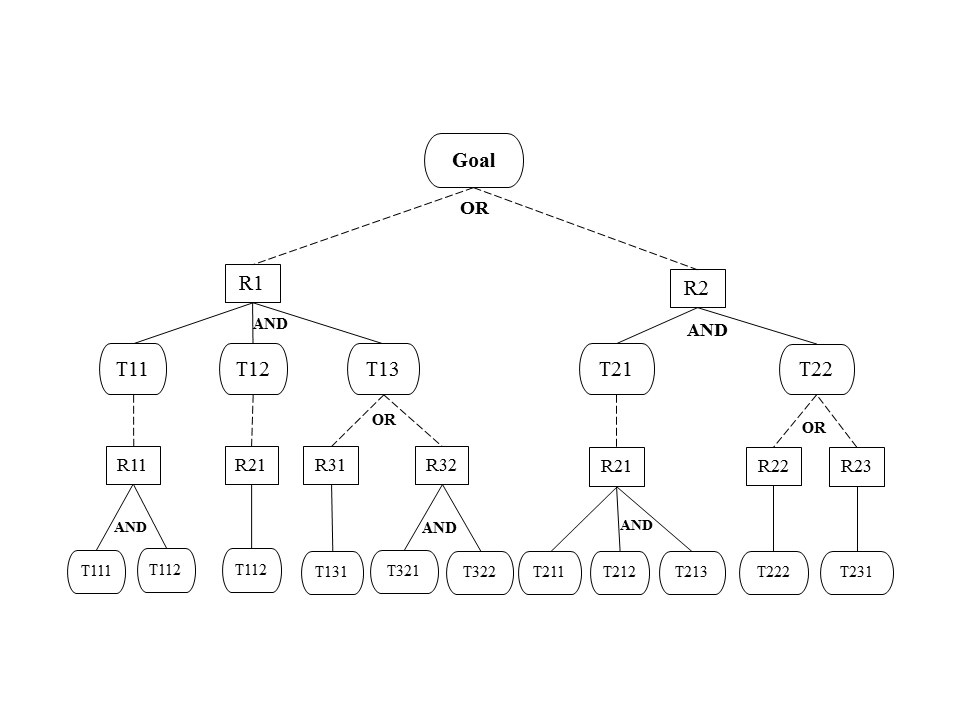
\includegraphics[width=\textwidth]{Pictures/htn1.png}
	\caption{\label{HTN tree representation} HTN tree representation}
\end{figure}


We denote two types of tasks; compound task or non-primitive task and primitive task or action. For example figure \ref{HTN example representation} represents a compound task Move (Obj, Room1, Room2, Door) which is decomposed into three primitive tasks $\{Pick-up (Obj), Walk (Room1, Room2, Door), Put-down(Obj)\}$.

\begin{figure}[h]
	\centering
	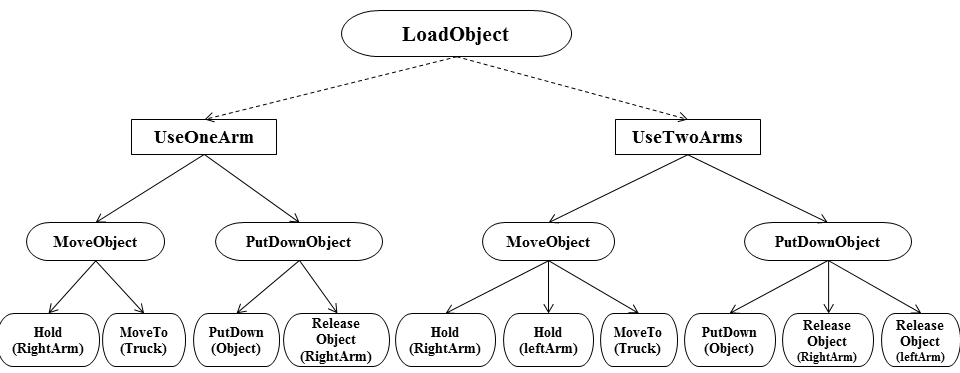
\includegraphics[width=\textwidth]{Pictures/example.png}
	\caption{\label{HTN example representation} HTN example representation}
\end{figure}


\subsubsection{HTN Recipe formalism}
An HTN recipe is used for decomposing compound tasks and has the form of a triple $\ R = (N, T, H)$ where $N$ is the name of the recipe which is unique such that no two recipes can have the same name. $T$ is a non-primitive task performed with this recipe and $H$ is a task network containing the set of subtasks of $T$, describing one way of performing the task T.


Using the HTN components formalism, we present now the domain knowledge and the HTN problem planning.

\par The Domain knowledge $D$ is a list of all the recipes in the HTN needed to decompose the HTN tasks. $\ D= [R1,. . . , Rn].$ Thus an HTN is a tree defined as a tuple $\ M =<T,D> $ where $T$ is the task network composed by all the tasks of the HTN and $D$ is the domain knowledge.

\par The planning problem $P$ is defined as a tree-tuple $\ P =< I, M, G>$ where $\ I$ is the initial state, $M$ is the domain problem defined by the HTN tree and $G$ is the goal task to achieve. $G$ belongs to the tasks of $M$ and the precondition of $G$ is true in $I$. The problem is to find a plan that solves $P$. HTN planning works by expanding tasks and resolving conflicts iteratively, until a conflict-free plan can be found that consists only of primitive tasks.

\par Planning proceeds using task decomposition that starts from the initial goal task $G$, expands this task using a corresponding recipe $R$, and breaks down the goal into sequence of simpler subtasks. This process is applied recursively until the planner reaches a sequence of fully ordered primitive tasks that can make a goal successful. Thus, the solution of the planning problem $P$ is a plan $\ \pi = [a1,.., an]$ is a sequence of primitive tasks $\ ai \in M$ , and $\ i \in [1,n].$

\par The HTN planners are becoming popular in different domains where several systems were developed these recent years such as SHOP \cite{nau1999shop}, SIPE \cite{wilkins1988practical} or NOAH \cite{sacerdoti1975structure}.

\par General purpose of planning as STRIPS and HTN relies on a complete model of the domain knowledge, that means if the model is not complete then, the planner won't be able to plan. This approach of planning is named \emph{Declarative representation}. Such representation of HTN requires a full modeling of HTN domain knowledge. Each
task in the HTN has at least one modeling specification that allows reasoning in planning. Despite the completeness of this representation, modeling such domain require significant knowledge-engineering effort if it is not impossible.

\section{Reactive HTNs}
Declarative approaches for planning attempt to predict the future. The planning is made in off-line phase that start from initial state to search for logical future states to reach a final goal state, using for that the modeling specifications in the domain knowledge. Once the plan is generated, the execution phase is launched in the environment.
\par In contrast with this approach, reactive HTNs propose an approach with no planning phase to predict the future states at all. Instead, they compute just the next task to perform in every instant. Moreover, because of the complexity of modeling a domain knowledge, reactive HTNs run through a hand-authored HTN with a procedural definition of the modeling specifications. Procedural definition of the domain knowledge means that the planner cannot reason about theses conditions, the conditions are script code (example JavaScript)  that can only be executed or evaluated in the current state.

\par The solution of a planning problem is to find a path through the HTN using recipe selection. Starting from the initial state and the goal task, The HTN incrementally generates a sequence of sub-goals by choosing recipes for decomposing tasks. The recipe is selected by the applicability condition at the state where this last can be evaluated. The modeling specifications are evaluated in the current state, if it returns the values true the HTN consider it as valid and continue the exploration of the HTN. However if the evaluation of any specification fails (returns false), the
HTN execution fails and we say that the HTN reaches a dead end. This situation is considered as hard failure. 

The execution is considered as complete if primitive tasks that make the goal successful are reached. Reactive HTN are becoming very popular in the field of controlling complex artificial intelligent systems exist performing in dynamic environment such as Dialog with the Disco system \cite{rich2009building} and RavenClaw \cite{bohus2003ravenclaw}.

\section{Plan execution, breakdown and recovery}
The declarative planners introduced before return a plan $\ \pi $ composed of a sequence of primitive tasks (actions), which is passed to the controller for the execution phase. The execution starts from the initial state and has to achieve the execution
of all the actions of the plan to reach the goal state. The execution of a STRIPS action is valid if its preconditions match subsets of the current observed world state immediately before the action is executed. The effects the executed action are added to the resulting state and the deleted effects are removed from it.

\par The HTN execution takes the STRIPS execution one step further by introducing the postcondition checks. As STRIPS primitive task (action) is applicable if its preconditions are valid in the current state of the world, in addition, the execution of the primitive task is considered as succeed only if its postconditions are part from the resulting state. Thus, the plan is a solution to a planning problem if it matches a subset of the current world state immediately after the last action in the plan is executed.

\par As the environment is dynamic, the controller monitors the environment at each execution step in order to prevent a breakdown. A breakdown occurs if any deviation from the steps defined in the constructed plan is detected, such deviation makes the executed plan invalid and the execution of plan stops. The breakdown
is identified if the world changes in an unexpected way that causes the execution failure of an action. The failure can be caused by one of these situations:
\begin{itemize}
	\item First, the action preconditions are no longer satisfied in the current state. For example, a robot that plans to walk from room1 to room2 through door1, arriving at door1 the wind blows and the door1 became close, this unexpected change invalidate the precondition of the action that is the door must be open.
	\item Second, the executed action leads to unexpected consequences, in this case the postconditions of the action are not satisfied.
\end{itemize}
%
\section{The problem}

Systems presented above need to plan, a complete definition of the domain knowledge which represent the real world faithfully. However,the dynamic definition of the environment in real problems implies unexpected changes that planner must predict and handle. For example, representing cooking problem such in Figure \ref{Cooking model example} involve representing all the actions and devices used. In addition, the model must contain tasks that can handle each change in the environment. For example, when modeling the cook task which involve heat the oven, if an electrical failure happens, then the planner has to react and restores electricity. However,  constructing such complete logical (declarative) model of real and complex problems that run in dynamic environment requires significant knowledge-engineering effort nearly impossible.  Thus, the domain knowledge is  incomplete which may lead the planner to face breakdowns. 
 \begin{figure}[h]
 	\centering
 	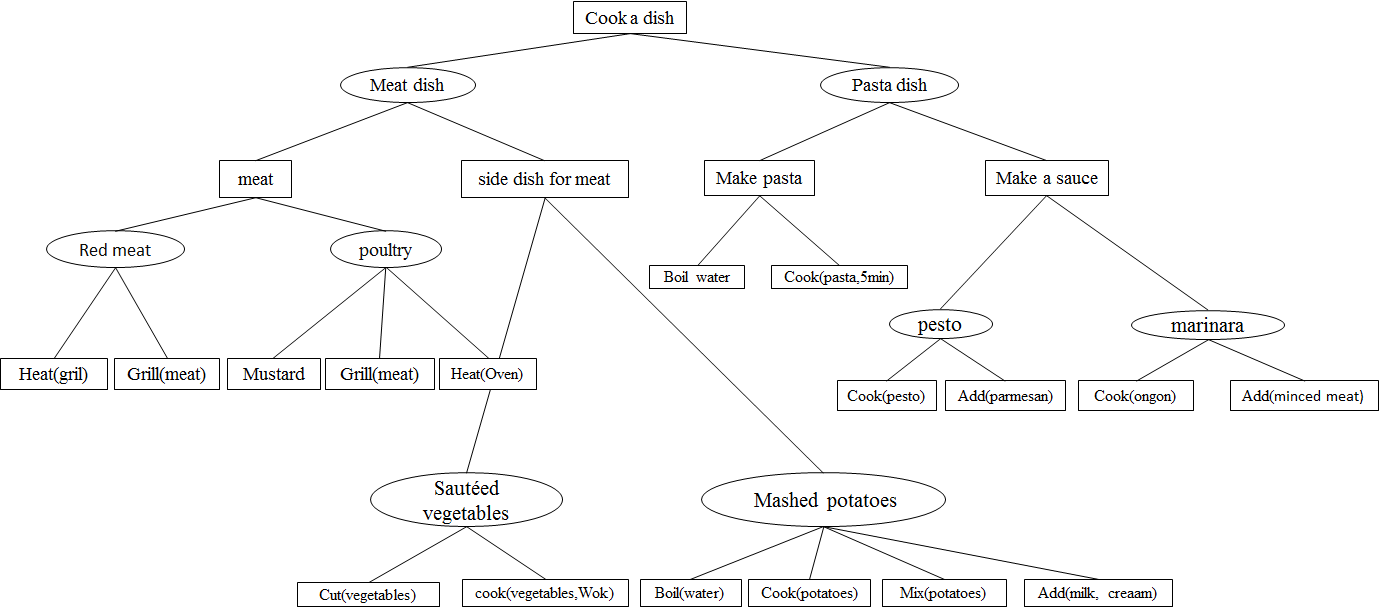
\includegraphics[width=\textwidth]{Pictures/cooking.png}
 	\caption{\label{Cooking model example} Cooking model example}
 \end{figure}
 

In addition, reactive HTNs take the position of using no planning process to detects the future state. Instead, the HTN plans only for the next task to be executed  based only on the current observable state. HTNs use procedural definition of the domain knowledge that can offer no reasoning and  uses an optimistic valuation of the conditions . This execution approach can lead the HTN to a state where no decomposition or execution are possible, this state is then called dead end. In such case, we say that the HTN executor faces a breakdown.Because of the procedural definition of the domain knowledge and the reactive formalism of the HTN, this later is unable to backtrack in order to find another way to achieve the goal task.
Therefore, the HTN can no longer continue its execution and the goal is impossible to achieve.

For example, lets the HTN describing the move\&paint task execution presented in Figure \ref{break example}. The HTN starts the decomposition from the top level goal and at each step it monitors the conditions of each task. Once it attempts primitive tasks, the execution in the real world starts. the HTN starts by executing the pickup(Object) task, by first evaluating its preconditions, after the execution of the task, the HTN evaluates its  postcondition. Arriving to the execution of the Walk task,  the world changes in unexpected way; assume that the wind blows and the door is now blocked.Thus, the preconditions of the Walk(room1, room2, door1) task (i.e IsOpen(Door)) are no longer valid. the HTN execution is then blocked and a breakdown is then detected.
 \begin{figure}[h]
 	\centering
 	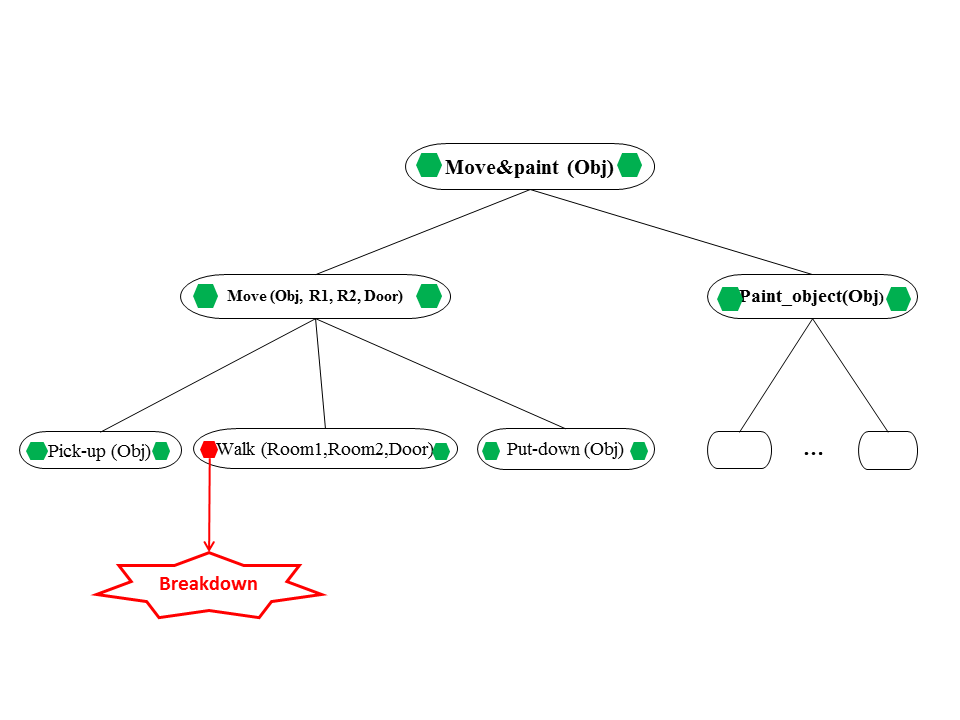
\includegraphics[width=\textwidth]{Pictures/break.png}
 	\caption{\label{break example} Breakdown situation in the move\&paint example}
 \end{figure}
 
 \section{Conclusion}
This chapter presented the background of our work.First, we presented and discussed the existing methods in the field of planning, from linear planning to hierarchical planning. Then we defined  the addressed problem which concerns breakdowns especially in reactive HTN, and the necessity of recovering from breakdowns taking in account the incompleteness of reactive HTN's knowledge domain.

In the next chapter (chapter3), we will put forward the existing approaches to recover from breakdowns and discuss their utility in the addressed problem. Next, we will present in chapter 4 the proposed solution to recover from breakdowns in reactive HTN with incomplete models and details the architecture of the plan recover system. 
 
\chapter{Discolog approach} % Main chapter title

\label{Chapter 4} % For referencing the chapter elsewhere, use \ref{Chapter1} 

 In this Chapter, we introduce the Discolog system, a reactive HTN planning, execution, and plan-repairing system. Discolog is a   hybrid system that integrates  a reasoning engine modeled by STRIPS planner to a reactive HTN. We will first present an overview of the system, and next we will detail the system architecture.
\lhead{Chapter 4. \emph{Discolog approach}}

%In this section, we introduce our solution for plan recovery in reactive HTN. We also %present the description of the main procedures of plan recovery algorithm.


 Discolog uses reactive HTN style to achieve a goal with no prediction of future states at all.
 Starting from the top level goal, Discolog recursively decomposes tasks until it reaches a set of primitives tasks that can be directelly executed in the real world. 

 Nevertheless, because of procedural definition of reactive HTN domain knowledge which doesn't contain any logical information allowing the planner reasoning about task decomposition and execution, if the HTN faces breakdowns during the execution, it will be unable to backtrack  finding another decomposition that achieves the execution of the task.
 
 
In order to face this problem, Discolog uses a STRIPS planner to propose a plan recovery. It starts from the current observable state of the world and uses only the partial information available in the domain knowledge of the HTN to reason about. For that matter, Discolog extends the definition of certain HTN tasks in the domain knowledge from procedural definition to a declarative definition . An overview of the proposed execution and plan repair system is illustrated in Figure ~\ref{High level description of Discolog system}  .
		\begin{figure}[!h]
			\centering
			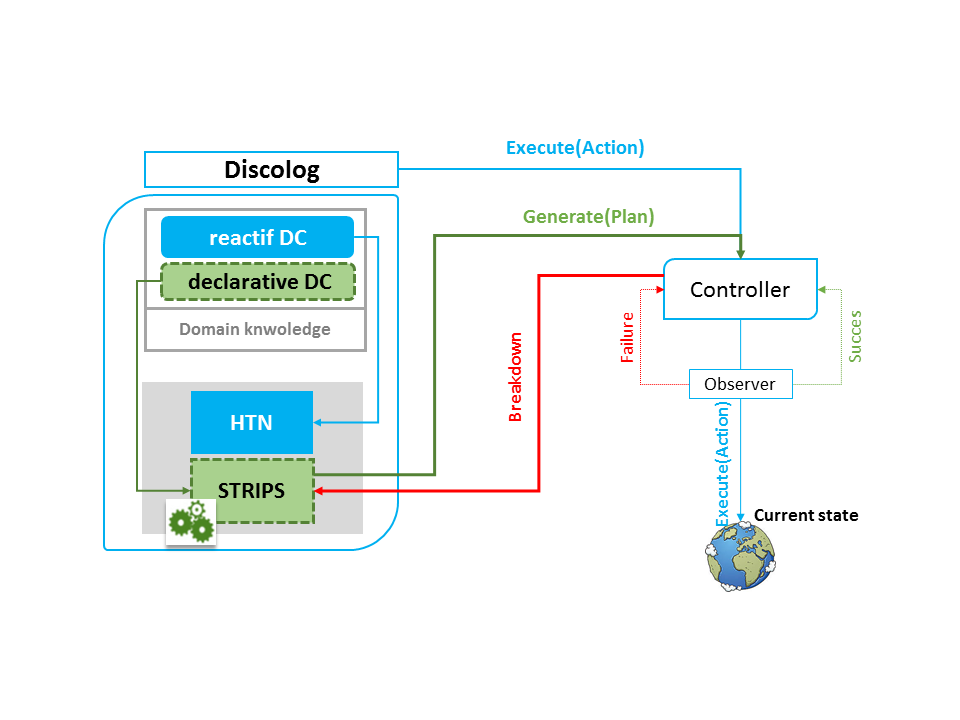
\includegraphics[width=250pt]{Pictures/architecture.png}
			\caption{\label{High level description of Discolog system} High level description of Discolog system}
		\end{figure}

The plan recovery in Discolog comprises two main procedures. The first one attempts to detect goal candidates to repair and the second invoke the STRIPS planner to propose a plan repair for these candidates. these procedures are described in the next sections.
\section{The Discolog algorithm}
Let \textit{HTN} be a model of an Hierarchical Task Network with a top level task \textit{Goal} to achieve, and Disco the the reactive HTN .To achieve \textit{Goal},  Disco  proceed as follow:
As showed in \ref{euclid}, Discolog starts from the top level goal \textit{Goal} and recursively decomposes tasks until it reaches a set of primitives tasks that can achieve \textit{Goal}.
Each task in Disco is defined with a \textit{status(Task)} $\in$ \{Live,Blocked,Done,Failed,Succeed\}.
\par Before decomposing a non primitive task or executing primitives task, Disco evaluate the precondition of the this task. If the current state holds the preconditions(Task) then status(Task) is updated to Live. otherwise, Status(Task)= not Live and the HTN execution is blocked.
The same, after the execution of a primitive task, Disco evaluate its postconditions. If postconditions(Task) are valid in the current state the status(Task) is updated to done or succeed, otherwise status(Task)= failed and the HTN execution become blocked.


At the end of the process, Disco(HTN,Goal) returns either Success(Goal is achieved) or failure if Disco faces breakdown. These breakdowns are detected if the top level goal is not achieved i.e Status(Goal) != Done and Disco has no decomposition or execution to propose. 

When such breakdown occurs, Discolog starts the recover procedure which will first look over the \textit{Goal} and its children to find task candidates which can be repaired from the current state in order to recover from the breakdown. The recover procedure is defined in the next sections.  
\begin{algorithm}
	\caption{DiscoLog algorithm }\label{euclid}
	\begin{algorithmic}[]
		\Procedure{Discolog}{HTN,Goal}
		\State $\textit{HTN} \gets\textit{ConstructModel()} $
		\State $\pi \gets Disco \textit{(HTN,Goal)}$
		\If {$ \pi \gets\textit{Success} $} 
		\State \Return $\textit{Success} $
		\Else 
		\State$ plan \gets Recover(Goal)$
		\If {(plan = \textit{null})}
		\State \Return Failure
		\Else 
		\For{$ \textbf{each}\text{ action }\textit{ai} \in plan $}
		\State  $\textit{Discolog} \text{(HTN,ai)}$
		\EndFor
		\EndIf
		\EndIf
		\\
		\EndProcedure \textbf{EndProcedure}
		\State 
		\Procedure{Recover}{Goal}
		\State $\textit{listCandidates}\gets\textit{findCandidate}{(G)} $
		\If {$ \textit{listCandidates = }\emptyset $} 
		\State \Return $\textit{null} $
		\Else 
		\State $\Pi \gets \emptyset$
		
		\For{$ \textbf{each} \textit{ candidate} \in \textit{listCandidates}$}
		\State $\Pi += InvokeSTRIPS(candidate,CurrentState)$
		\State  $Cost \gets \{ cost(\pi) | \pi \in  \Pi \} $
		\EndFor
		\EndIf
		\State \Return $\pi \in \Pi \text{ with minimum cost}(\pi)$
		\\
		\EndProcedure \textbf{EndProcedure}
		
		\State 
		\Procedure{FindCandidate}{Goal}
		\For{$ \textbf{each} \textit{ child} \in \textit{Goal}$}
		
		\If {$\text{(precondition(child)!=} \emptyset \text{ and}$
			\State$ \textbf{ status} (child)\notin\{\text{Done, Live, Blocked}\})$}
		\State $  \text{ add precondition(child) to candidates}$
		
		\ElsIf{$\text{(postcondition(child)!=}\emptyset 
			\text{ and } \textbf{ status} \text{(child)} \in \{\text{Failed}\}$}
		\State $\text{add postcondition(child) to candidates}$
		\EndIf
		\If {$(\textbf{status} \in \{\text{Live}\}\text{ and nonprimitive(child) and applicability(child)!=}\emptyset)$}
		\State add Applicabilitcondition(child) to candidates
		\EndIf
		\State $\textit{findCandidate} (children(child))$
		\EndFor
		\State \Return candidates
		\\
		\EndProcedure \textbf{EndProcedure}
		
	\end{algorithmic}
\end{algorithm}
\subsection{Goal candidates detection}
When a breakdown occurs, Discolog  will  first look over the goal task and its children to determine tasks in the HTN which are compromised by the breakdown, theses tasks are defined as task candidates for the plan recovery. 
For each task, we extract the condition failed because of the breakdown: 
\begin{itemize}
	\item	If the status of task is neither done nor live then the algorithm will attempts to repair its preconditions
	\item	If the status of task is failed then its postcondition are not valid and the repair algorithm will attempts to repair these postconditions.
	\item	if the task is nonprimitive and all its applicability conditions are invalid in the current state then the algorithm will attempts te replan to satisfy one of its applicability condition. 
\end{itemize}

Once, the list of candidate is identified, it is then passed to the InvokeStrips procedure.
As presented previously, a breakdown occur in a HTN if one of the task conditions fails, thus repairing a task using STRIPS planner is considered as repairing the failed condition of this task.
Once, the list of candidate is identified, the prolog STRIPS planner is called to propose a recovery plan.
\subsection{STRIPS repair planner}
In order to generate a plan, STRIPS has to constitute the planning problem to reason about. First  STRIPS constructs its domain knowledge by extracting partial information from the HTN domain knowledge and extends them to declarative definition. For that, Discolog convert all the primitive tasks to a declarative and logical formalism supported by STRIPS. Then for each candidate task, STRIPS takes as goal state  the failed task condition of the task candidate  and the current observable state is defined as the initial state.

Next, STRIPS tries to generate a linear plan to failed condition to reach a state where the failed condition is valid. Finally, Discolog calculate the best. i.e the  plan the plan with the minimum cost of execution and convert its actions to reactive formalism. this plan is then passed to Disco to be executed in the environment.

\section{Example}

Lets the HTN describing the move\&paint task execution presented in figure \ref{Plan recovery}. The HTN starts the decomposition from the top level goal and at each step it monitors the conditions of each task. Once it attempts primitive tasks, the execution in the real world starts. the HTN starts by executing the pickup(Object) by first evaluating its preconditions, after the execution of the task, the HTN evaluated the postconditions of the task. Arriving to the execution of the Walk task, , the world suddenly changes; assume that the wind blows and the door is now blocked thus the preconditions of the Walk(room1, room2, door1) task are no longer valid. Then a breakdown is detected and the recover procedure is called.


To recover from this breakdown, Discolog will first define the task candidates that can be repaired, which are the walk task with its preconditions and the move task with its postconditions. 

Once the list defined, it is passed to the STRIPS planner, which creates its domain knowledge as shown in figure \ref{Plan recovery}, next it generates a plan for both candidates. STRIPS returns the best plan that can repair the walk task composed. In this example the best plan consists of two primitives tasks; unlock(door) and open(door). 
This plan is converted to Disco tasks and executed. Once the plan recovery executed, Discolog continue the task decomposition from the current state to achieve the moveandpaint task. 

		\begin{figure}[h]
			\centering
			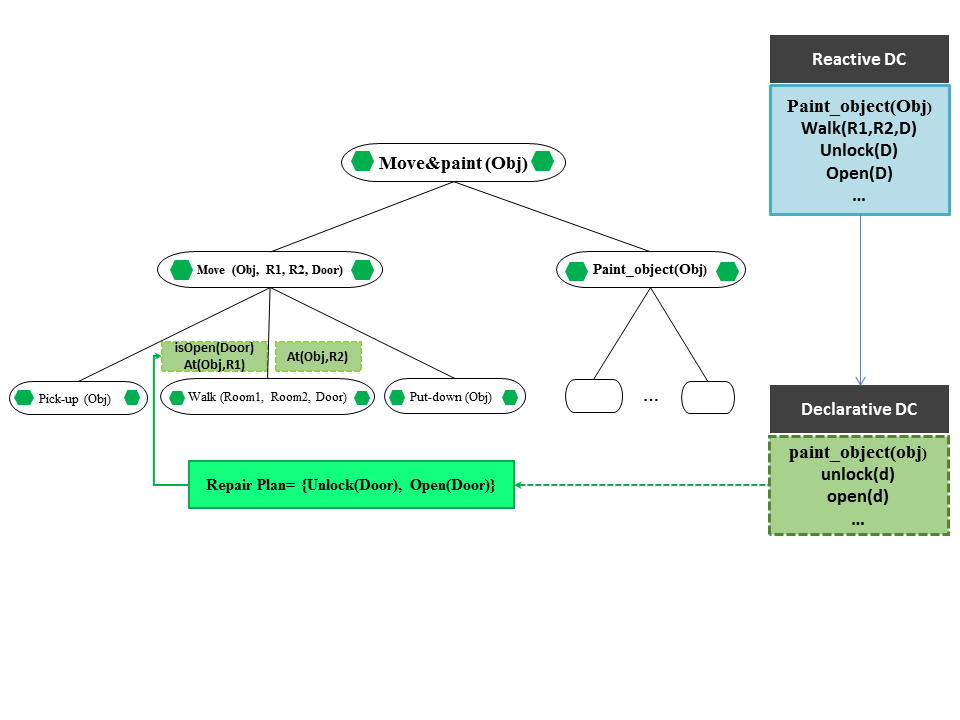
\includegraphics[width=.75\columnwidth]{Pictures/repair.png}
			\caption{\label{Plan recovery} Plan recovery for the move\&paint task using Discolog}
		\end{figure}
		
We present in this chapter the proposed solution and we detailed the conceptional procedure of this later. In the next chapter, we will present the implementation of the Discolog system.
%Let \textit{HTN} be a model of an Hierarchical Task Network with a top level task \textit{Goal} to achieve.To achieve \textit{Goal} Disco proceed as follow:
%
%
%Starting from the top level goal \textit{Goal}, Disco recursively decomposes tasks until it reaches a set of primitives tasks that can be directelly executed in the real world to achieve \textit{Goal}.
%Each task in Disco has a \textit{status(Task)} $\in$ \{Live,Blocked,Done,Failed,Succeed\}.
%\par Before decomposing a non primitive task or executing primitives task, Disco evaluate the precondition of the this task. If the current state holds the preconditions(Task) then status(Task) is updated to Live. otherwise, Status(Task)= Blocked and the HTN execution is blocked.
%The same, after the execution of a primitive task(execution of the grounding script), Disco evaluate its postconditions. If postconditions(Task) are valid in the current state the status(Task) is updated to done or succeed, otherwise status(Task)= failed and the HTN execution become blocked.
%\section{Description of the algorithm \ref{euclid}}
%
%
%At the end of the process, Disco(HTN,Goal) returns either Success(Goal is achieved) or failure if Disco faces breakdown. These breakdowns are detected if the top level goal is not achieved i.e Status(Goal) != Done and Disco has no decomposition or execution to propose. 
%
%When such breakdown occurs, the recovery algorithm will, first look over the \textit{Goal} and its children to find task candidates which can be repaired from the current state in order to recover from the breakdown. This process is handled by the procedure FindCandidates() described in the Algorithm \ref{euclid}.
% :
%\begin{itemize}
%	\item	If the status of task is neither done nor live then the algorithm will attempts to repair its preconditions
%	\item	If the status of task is failed then its postcondition are not valid and the repair algorithm will attempts to repair these postconditions.
%	\item	if the task is nonprimitive and all its applicability conditions are invalid in the current state then the algorithm will attempts te replan to satisfy one of its applicability condition. 
%\end{itemize}
%
%For example, the moveandpaint task which breakdowns in the execution of the walk task because its precondition "isOpen(door)" is no longer valid in the current state. 
%
%Once, the list of candidate is identified, the prolog STRIPS planner is called for each candidate and the solution with the shorter plan is returned to Disco to be executed in the real world.


% Chapter 1

\chapter{Implementation} % Main chapter title

\label{Chapter 5} % For referencing the chapter elsewhere, use \ref{Chapter1} 

\lhead{Chapter 5. \emph{Implementation}} % This is for the header on each page - perhaps a shortened title
We described in previous chapters of this thesis, the  problem  being addressed and our proposition for a solution. In the following, we present the implementation of this solution. 

\section{Development environment }
In order to implement the hybrid system Discolog, we used the collaborative discourse engine Disco \cite{rich2009building} as reactive HTN to which we integrate a Prolog STRIPS planner  to support the plan repair process. 

The most important challenge within the realization of such hybrid system is to support heterogeneous formalisms of Disco and STRIPS. The system must be able to convert  the HTN domain knowledge from procedural formalism implemented in Java to a declarative one capable to run in Prolog  and  handle exceptions related to this conversion. 

For that purpose, we integrated to Disco the tuProlog \footnote{\url{http://apice.unibo.it/xwiki/bin/view/Tuprolog/}}  java-based light-weight Prolog engine to create a bridge that can use the logical Prolog planner from the Java procedural environment . the environment architecture is described  in figure \ref{implementation environment of Discolog}.
\begin{figure}[h]
	\centering
	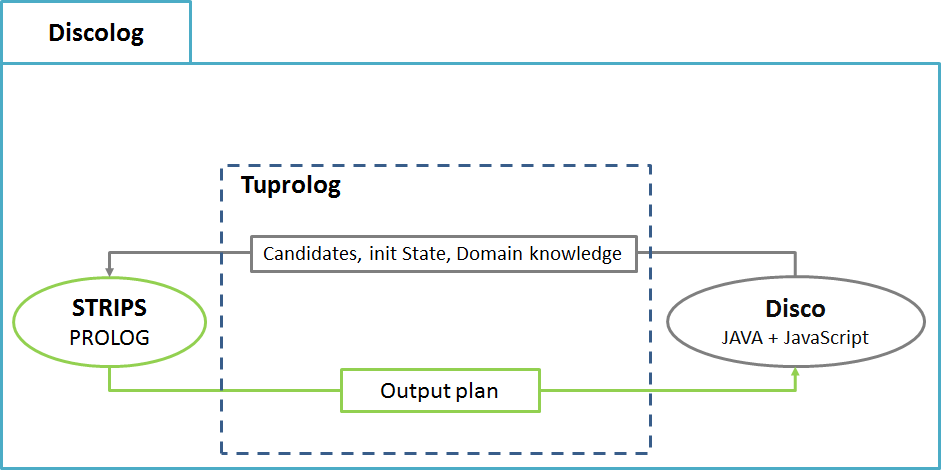
\includegraphics[width=\textwidth]{Pictures/archi1.png}
	\caption{\label{implementation environment of Discolog} implementation environment of Discolog}
\end{figure}


\section{Disco}
Disco \cite{rich2009building}is a collaborative discourse engine using reactive HTNS. The  most important feature of this reactive architecture is that allows the system to lead the user in a real time, without making any plan in advance. Disco's functional architecture is composed by a main component called \textit{task engine}. 
The function of the \textit{task engine}  is to load and validate a task model description and to maintain a representation of the current status of the user’s tasks.\cite{rich2009building}  


%----------------------------------------------------------------------------------------
\subsection{Disco task model}
Disco uses the ANSI/CEA-2018 standard for the procedural definition of the task model elements as described bellow :
\begin{itemize}
	\item \textit{Task}: The task model defines Task classes which are modeled using XML format, an example of the move\&paint implementation is showed in Appendix \ref{xml}. Primitive tasks may contain \textit{grounding script} parameter defined as JavaScript program which represent the effect of  the primitive task execution in the environment.
	
	\item \textit{Inputs and outputs} : Input includes all the data that may affect the execution of the task and output includes all data that can be affected by the execution of the task. these data type is defined in JavaScript.
	\item \textit{Conditions} : Task's conditions (Preconditions, postconditions ans applicability conditions) are defined as boolean JavaScript function to evaluate the execution of a task.

\end{itemize}

\section{Discolog implementation}
For the implementation of the Discolog system, we  faced some challenges. In addition to the management of heterogeneous environment, defining the level of information necessary to introduce in STRIPS domain knowledge required some reflection and designing a STRIPS planning algorithm able to provide effective solutions based on incomplete information in dynamic environment.
\subsection{The new Discolog API}
In order to implement the hybrid system Discolog we create an new  API divided in two mains folders :
	\begin{figure}[!h]
		\centering
		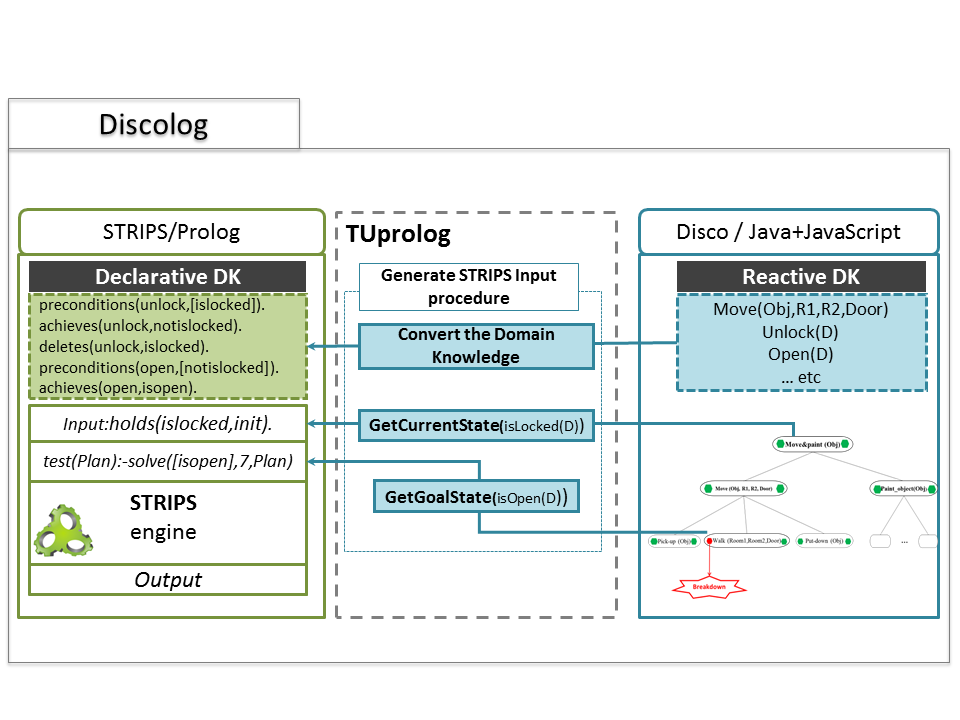
\includegraphics[width=\textwidth]{Pictures/input1.png}
		\caption{\label{input} Disco data generation in the moveandpaint example}
	\end{figure}
	
\subsubsection{ Disco extension }
We create an extension of Disco that can detect breakdowns and in such case, collects a candidates list for the plan recovery process. In addition, we manage to generate these candidates in the easiest way to be converted into Prolog formalism. The input Prolog planner is constituted in Disco via tuProlog as demonstrated in Figure \ref{input}.


 First, we start by creating the Prolog domain knowledge. Therefore, we extract all the primitives tasks and turn them to a Prolog formalism using tuProlog. Next, Disco observe the current state and convert it to the initial state. for example, in the move\&paint example, the current state where the breakdown occurs was IsLocked(Door) "the door is locked". Finally, the list of candidates is generated and each candidate is converted to a goal state to be achieve in Prolog.


\subsubsection{ Declarative Prolog implementation }
The main challenge faced in the creation of the STRIPS planner was to create an efficient means-end planning algorithm that can be integrated and executed  into tuProlog. Moreover, we had to define adequate structures that can receive the extracted domain knowledge. the STRIPS planner implemented is explained in Appendix \ref{AppendixB}.
% reference de STRIPS 


 Once STRIPS generate the plan recover, each action of this plan must be converted into primitive task formalism supported by Disco. Therefore we create a procedure that treat and convert the STRIPS plan output. An example of this procedure is shown  in Figure \ref{output} which describe how the plan repair is extracted for the move\&paint example. 

	\begin{figure}[!h]
		\centering
		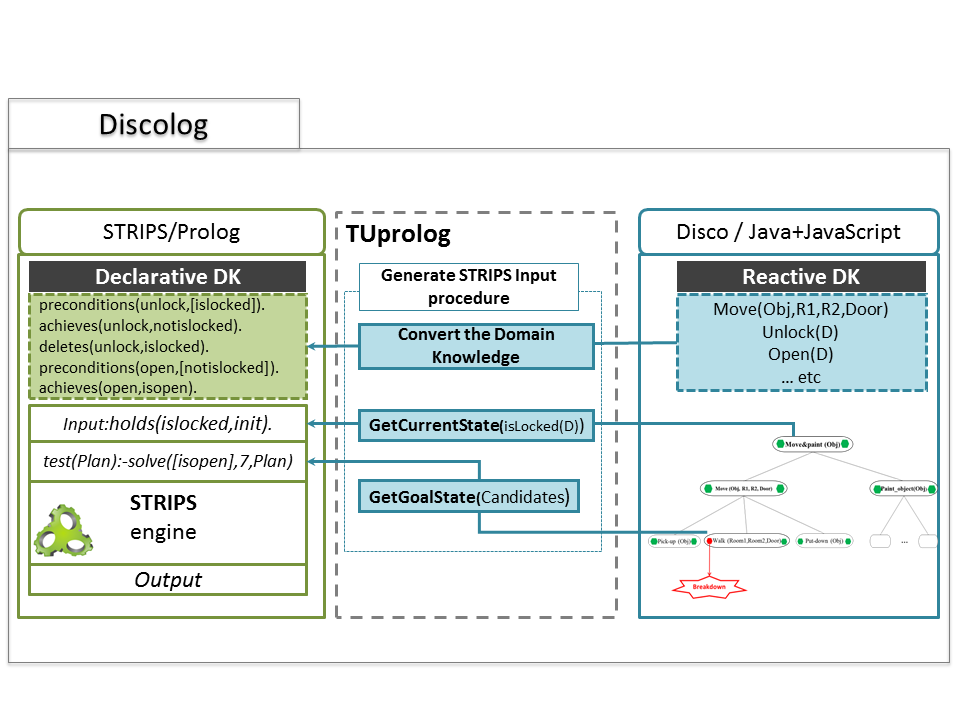
\includegraphics[width=\textwidth]{Pictures/output1.png}
		\caption{\label{output} Prolog data generation in the moveandpaint example}
	\end{figure}

\section{Conclusion}
In this chapter, we described the implementation of the Discolog system. First we introduce the environment of the implementation and we introduced the Disco system. Next we bring forward the new implemented Discolog API and explain each parts of this later.

In the next chapter, we present the experiments conducted to validate our system. 

%----------------------------------------------------------------------------------------


%\begin{multicols}{2}
%\lstinputlisting[language=XML]{Chapters/moveandpaint.xml}
%\end{multicols}
%\lstinputlisting[language=XML]{Chapters/moveandpaint.xml}

\chapter{Experiments, test and results} % Main chapter title

\label{Chapter 6} % For referencing the chapter elsewhere, use \ref{Chapter1} 

\lhead{Chapter 6. \emph{Experiments, test and results}}
The experimental evaluation was devised in two mains parts, the first consisted on constructing the HTN model to evaluate the Discolog system. The second point was to variate the level of knowledge to test the robustness of  Discolog system against different types of breakdown. 
%\section{experimental environment}

\section{experimental model creation}
In order to test efficiently the Discolog system, we must test the Discolog system on different type of HTN. in the absence of accurate models. we had to create our own evaluation data. Therefore, an algorithm was constructed to generate different types of HTN models. 

The evaluation HTN was constructed using synthetic data as demonstrated in the algorithm ...
\begin{itemize}
	\item Each compound task in the HTN has a set of [$r_1$, ...,$r_\text{recipes}$].
	\item Each recipe is constituted by [$r_1$, ...,$r_\text{length}$] children to decompose the parent task.
	\item the preconditions of the first child are the same as its parent, and the postconditions of the last child are the same as its parent. 
	\item Conditions defined in the primitive tasks are chained in each recipe. Example: the task a is decomposed to \{$a_1$, $a_2$, $a_3$\}using the recipe R1. Thus, the preconditions of $a_1$ are the same as its parent a and the postconditions of $a_3$ are the same as its parent a. We define the postcondition of $a_1$ as "P1" then the preconditions of the next task $a_2$ are "P1", we also define the postconditions of $a_2$ as "P2" then the preconditions of $a_3$ task are "P2".
	\item each recipe has its applicability condition, therefore, we generated primitives tasks whose postconditions turns to true the applicability condition of each recipe, in order to be able to recover from a breakdown caused by an applicability condition failure. 
\end{itemize}
\begin{algorithm}
\caption{DiscoLog algorithm }\label{tree}
\begin{algorithmic}[]
	\Procedure{CreateHTN}{depth,length,recipes,top}
	\State $\textit{ConstructHTNTree(depth,length,recipes,top)} $

	\State $\textit{DefineLevelOfKnwoledge(top, level)} $
	\EndProcedure \textbf{EndProcedure}
	\State
	\State
	
	\Procedure{ConstructHTNTree}{depth,length,recipes,top}
	\If {$\textit{depth} > 1 $}
\For{$ \textbf{each r} \in \text{ recipes} $}
\State $\text{addRecipe(r, top)}$
\For{$ \textbf{each l} \in \text{ length} $}
\State $\text{addchild(top,childl})$
\State $ConstructHTNTree(depth,length,recipes,childl)$
\EndFor
\EndFor
\EndIf
	\EndProcedure \textbf{EndProcedure}
\end{algorithmic}
\end{algorithm}
\subsection{Test algorithm}
The Discolog system was tested on each generated model several times, and for each model, we variate the type of breakdown to recover from and the level of knowledge used in the model. We calculate the percentage of recover relative to the level of knowledge. The generated algorithm is described bellow.
\begin{algorithm}
	\caption{Test algorithm }\label{test}
	\begin{algorithmic}[]
		\Loop \text{ (10) }
\Loop (\text{Random breakdowns } $\gets$ 100)
\State(Discolog(HTN,Goal))

\EndLoop\textbf{EndLoop} \\
\EndLoop\textbf{EndLoop} \\
	\end{algorithmic}
\end{algorithm}
 
\section{ results of the Experiments}
%\chapter{Discolog approach} % Main chapter title

\label{Chapter 4} % For referencing the chapter elsewhere, use \ref{Chapter1} 

 In this Chapter, we introduce the Discolog system, a reactive HTN planning, execution, and plan-repairing system. Discolog is a   hybrid system that integrates  a reasoning engine modeled by STRIPS planner to a reactive HTN. We will first present an overview of the system, and next we will detail the system architecture.
\lhead{Chapter 4. \emph{Discolog approach}}

%In this section, we introduce our solution for plan recovery in reactive HTN. We also %present the description of the main procedures of plan recovery algorithm.


 Discolog uses reactive HTN style to achieve a goal with no prediction of future states at all.
 Starting from the top level goal, Discolog recursively decomposes tasks until it reaches a set of primitives tasks that can be directelly executed in the real world. 

 Nevertheless, because of procedural definition of reactive HTN domain knowledge which doesn't contain any logical information allowing the planner reasoning about task decomposition and execution, if the HTN faces breakdowns during the execution, it will be unable to backtrack  finding another decomposition that achieves the execution of the task.
 
 
In order to face this problem, Discolog uses a STRIPS planner to propose a plan recovery. It starts from the current observable state of the world and uses only the partial information available in the domain knowledge of the HTN to reason about. For that matter, Discolog extends the definition of certain HTN tasks in the domain knowledge from procedural definition to a declarative definition . An overview of the proposed execution and plan repair system is illustrated in Figure ~\ref{High level description of Discolog system}  .
		\begin{figure}[!h]
			\centering
			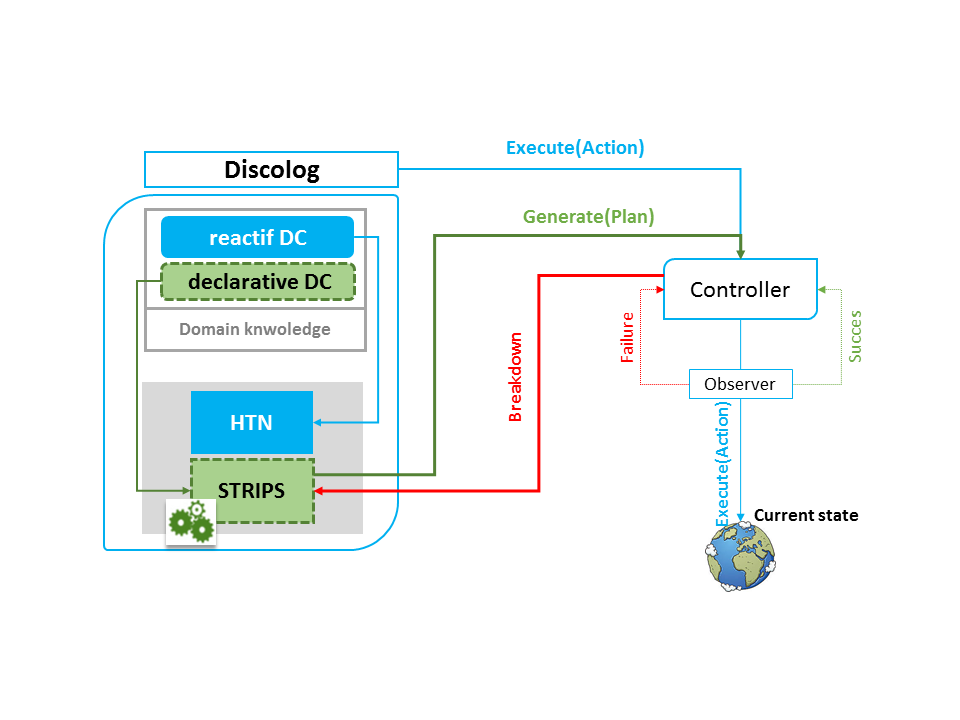
\includegraphics[width=250pt]{Pictures/architecture.png}
			\caption{\label{High level description of Discolog system} High level description of Discolog system}
		\end{figure}

The plan recovery in Discolog comprises two main procedures. The first one attempts to detect goal candidates to repair and the second invoke the STRIPS planner to propose a plan repair for these candidates. these procedures are described in the next sections.
\section{The Discolog algorithm}
Let \textit{HTN} be a model of an Hierarchical Task Network with a top level task \textit{Goal} to achieve, and Disco the the reactive HTN .To achieve \textit{Goal},  Disco  proceed as follow:
As showed in \ref{euclid}, Discolog starts from the top level goal \textit{Goal} and recursively decomposes tasks until it reaches a set of primitives tasks that can achieve \textit{Goal}.
Each task in Disco is defined with a \textit{status(Task)} $\in$ \{Live,Blocked,Done,Failed,Succeed\}.
\par Before decomposing a non primitive task or executing primitives task, Disco evaluate the precondition of the this task. If the current state holds the preconditions(Task) then status(Task) is updated to Live. otherwise, Status(Task)= not Live and the HTN execution is blocked.
The same, after the execution of a primitive task, Disco evaluate its postconditions. If postconditions(Task) are valid in the current state the status(Task) is updated to done or succeed, otherwise status(Task)= failed and the HTN execution become blocked.


At the end of the process, Disco(HTN,Goal) returns either Success(Goal is achieved) or failure if Disco faces breakdown. These breakdowns are detected if the top level goal is not achieved i.e Status(Goal) != Done and Disco has no decomposition or execution to propose. 

When such breakdown occurs, Discolog starts the recover procedure which will first look over the \textit{Goal} and its children to find task candidates which can be repaired from the current state in order to recover from the breakdown. The recover procedure is defined in the next sections.  
\begin{algorithm}
	\caption{DiscoLog algorithm }\label{euclid}
	\begin{algorithmic}[]
		\Procedure{Discolog}{HTN,Goal}
		\State $\textit{HTN} \gets\textit{ConstructModel()} $
		\State $\pi \gets Disco \textit{(HTN,Goal)}$
		\If {$ \pi \gets\textit{Success} $} 
		\State \Return $\textit{Success} $
		\Else 
		\State$ plan \gets Recover(Goal)$
		\If {(plan = \textit{null})}
		\State \Return Failure
		\Else 
		\For{$ \textbf{each}\text{ action }\textit{ai} \in plan $}
		\State  $\textit{Discolog} \text{(HTN,ai)}$
		\EndFor
		\EndIf
		\EndIf
		\\
		\EndProcedure \textbf{EndProcedure}
		\State 
		\Procedure{Recover}{Goal}
		\State $\textit{listCandidates}\gets\textit{findCandidate}{(G)} $
		\If {$ \textit{listCandidates = }\emptyset $} 
		\State \Return $\textit{null} $
		\Else 
		\State $\Pi \gets \emptyset$
		
		\For{$ \textbf{each} \textit{ candidate} \in \textit{listCandidates}$}
		\State $\Pi += InvokeSTRIPS(candidate,CurrentState)$
		\State  $Cost \gets \{ cost(\pi) | \pi \in  \Pi \} $
		\EndFor
		\EndIf
		\State \Return $\pi \in \Pi \text{ with minimum cost}(\pi)$
		\\
		\EndProcedure \textbf{EndProcedure}
		
		\State 
		\Procedure{FindCandidate}{Goal}
		\For{$ \textbf{each} \textit{ child} \in \textit{Goal}$}
		
		\If {$\text{(precondition(child)!=} \emptyset \text{ and}$
			\State$ \textbf{ status} (child)\notin\{\text{Done, Live, Blocked}\})$}
		\State $  \text{ add precondition(child) to candidates}$
		
		\ElsIf{$\text{(postcondition(child)!=}\emptyset 
			\text{ and } \textbf{ status} \text{(child)} \in \{\text{Failed}\}$}
		\State $\text{add postcondition(child) to candidates}$
		\EndIf
		\If {$(\textbf{status} \in \{\text{Live}\}\text{ and nonprimitive(child) and applicability(child)!=}\emptyset)$}
		\State add Applicabilitcondition(child) to candidates
		\EndIf
		\State $\textit{findCandidate} (children(child))$
		\EndFor
		\State \Return candidates
		\\
		\EndProcedure \textbf{EndProcedure}
		
	\end{algorithmic}
\end{algorithm}
\subsection{Goal candidates detection}
When a breakdown occurs, Discolog  will  first look over the goal task and its children to determine tasks in the HTN which are compromised by the breakdown, theses tasks are defined as task candidates for the plan recovery. 
For each task, we extract the condition failed because of the breakdown: 
\begin{itemize}
	\item	If the status of task is neither done nor live then the algorithm will attempts to repair its preconditions
	\item	If the status of task is failed then its postcondition are not valid and the repair algorithm will attempts to repair these postconditions.
	\item	if the task is nonprimitive and all its applicability conditions are invalid in the current state then the algorithm will attempts te replan to satisfy one of its applicability condition. 
\end{itemize}

Once, the list of candidate is identified, it is then passed to the InvokeStrips procedure.
As presented previously, a breakdown occur in a HTN if one of the task conditions fails, thus repairing a task using STRIPS planner is considered as repairing the failed condition of this task.
Once, the list of candidate is identified, the prolog STRIPS planner is called to propose a recovery plan.
\subsection{STRIPS repair planner}
In order to generate a plan, STRIPS has to constitute the planning problem to reason about. First  STRIPS constructs its domain knowledge by extracting partial information from the HTN domain knowledge and extends them to declarative definition. For that, Discolog convert all the primitive tasks to a declarative and logical formalism supported by STRIPS. Then for each candidate task, STRIPS takes as goal state  the failed task condition of the task candidate  and the current observable state is defined as the initial state.

Next, STRIPS tries to generate a linear plan to failed condition to reach a state where the failed condition is valid. Finally, Discolog calculate the best. i.e the  plan the plan with the minimum cost of execution and convert its actions to reactive formalism. this plan is then passed to Disco to be executed in the environment.

\section{Example}

Lets the HTN describing the move\&paint task execution presented in figure \ref{Plan recovery}. The HTN starts the decomposition from the top level goal and at each step it monitors the conditions of each task. Once it attempts primitive tasks, the execution in the real world starts. the HTN starts by executing the pickup(Object) by first evaluating its preconditions, after the execution of the task, the HTN evaluated the postconditions of the task. Arriving to the execution of the Walk task, , the world suddenly changes; assume that the wind blows and the door is now blocked thus the preconditions of the Walk(room1, room2, door1) task are no longer valid. Then a breakdown is detected and the recover procedure is called.


To recover from this breakdown, Discolog will first define the task candidates that can be repaired, which are the walk task with its preconditions and the move task with its postconditions. 

Once the list defined, it is passed to the STRIPS planner, which creates its domain knowledge as shown in figure \ref{Plan recovery}, next it generates a plan for both candidates. STRIPS returns the best plan that can repair the walk task composed. In this example the best plan consists of two primitives tasks; unlock(door) and open(door). 
This plan is converted to Disco tasks and executed. Once the plan recovery executed, Discolog continue the task decomposition from the current state to achieve the moveandpaint task. 

		\begin{figure}[h]
			\centering
			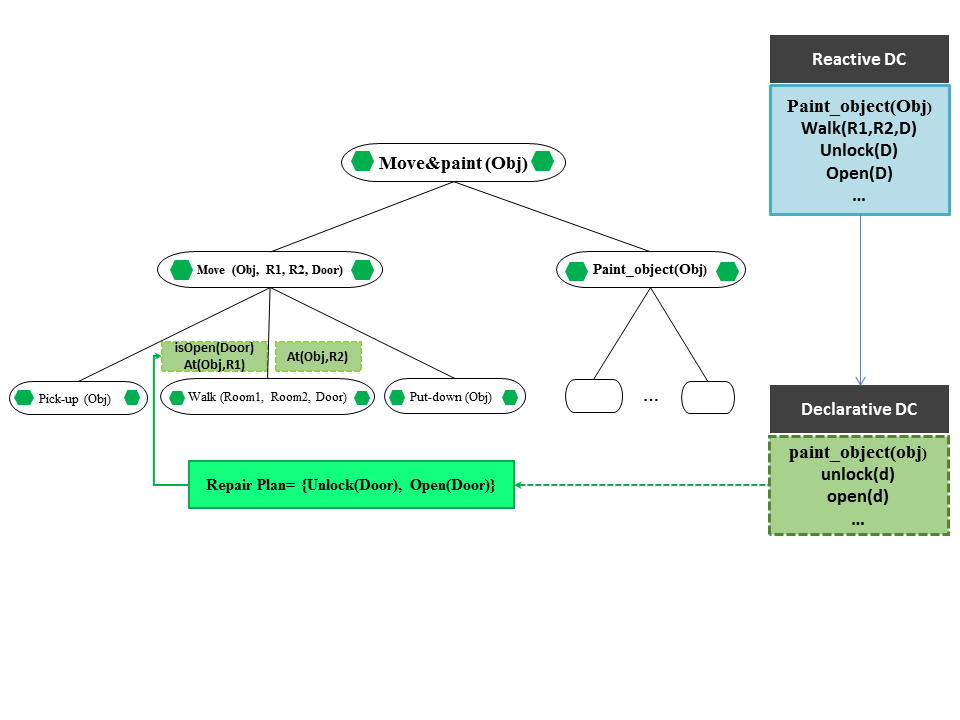
\includegraphics[width=.75\columnwidth]{Pictures/repair.png}
			\caption{\label{Plan recovery} Plan recovery for the move\&paint task using Discolog}
		\end{figure}
		
We present in this chapter the proposed solution and we detailed the conceptional procedure of this later. In the next chapter, we will present the implementation of the Discolog system.
%Let \textit{HTN} be a model of an Hierarchical Task Network with a top level task \textit{Goal} to achieve.To achieve \textit{Goal} Disco proceed as follow:
%
%
%Starting from the top level goal \textit{Goal}, Disco recursively decomposes tasks until it reaches a set of primitives tasks that can be directelly executed in the real world to achieve \textit{Goal}.
%Each task in Disco has a \textit{status(Task)} $\in$ \{Live,Blocked,Done,Failed,Succeed\}.
%\par Before decomposing a non primitive task or executing primitives task, Disco evaluate the precondition of the this task. If the current state holds the preconditions(Task) then status(Task) is updated to Live. otherwise, Status(Task)= Blocked and the HTN execution is blocked.
%The same, after the execution of a primitive task(execution of the grounding script), Disco evaluate its postconditions. If postconditions(Task) are valid in the current state the status(Task) is updated to done or succeed, otherwise status(Task)= failed and the HTN execution become blocked.
%\section{Description of the algorithm \ref{euclid}}
%
%
%At the end of the process, Disco(HTN,Goal) returns either Success(Goal is achieved) or failure if Disco faces breakdown. These breakdowns are detected if the top level goal is not achieved i.e Status(Goal) != Done and Disco has no decomposition or execution to propose. 
%
%When such breakdown occurs, the recovery algorithm will, first look over the \textit{Goal} and its children to find task candidates which can be repaired from the current state in order to recover from the breakdown. This process is handled by the procedure FindCandidates() described in the Algorithm \ref{euclid}.
% :
%\begin{itemize}
%	\item	If the status of task is neither done nor live then the algorithm will attempts to repair its preconditions
%	\item	If the status of task is failed then its postcondition are not valid and the repair algorithm will attempts to repair these postconditions.
%	\item	if the task is nonprimitive and all its applicability conditions are invalid in the current state then the algorithm will attempts te replan to satisfy one of its applicability condition. 
%\end{itemize}
%
%For example, the moveandpaint task which breakdowns in the execution of the walk task because its precondition "isOpen(door)" is no longer valid in the current state. 
%
%Once, the list of candidate is identified, the prolog STRIPS planner is called for each candidate and the solution with the shorter plan is returned to Disco to be executed in the real world.

 
%% Chapter 1

\chapter{Implementation} % Main chapter title

\label{Chapter 5} % For referencing the chapter elsewhere, use \ref{Chapter1} 

\lhead{Chapter 5. \emph{Implementation}} % This is for the header on each page - perhaps a shortened title
We described in previous chapters of this thesis, the  problem  being addressed and our proposition for a solution. In the following, we present the implementation of this solution. 

\section{Development environment }
In order to implement the hybrid system Discolog, we used the collaborative discourse engine Disco \cite{rich2009building} as reactive HTN to which we integrate a Prolog STRIPS planner  to support the plan repair process. 

The most important challenge within the realization of such hybrid system is to support heterogeneous formalisms of Disco and STRIPS. The system must be able to convert  the HTN domain knowledge from procedural formalism implemented in Java to a declarative one capable to run in Prolog  and  handle exceptions related to this conversion. 

For that purpose, we integrated to Disco the tuProlog \footnote{\url{http://apice.unibo.it/xwiki/bin/view/Tuprolog/}}  java-based light-weight Prolog engine to create a bridge that can use the logical Prolog planner from the Java procedural environment . the environment architecture is described  in figure \ref{implementation environment of Discolog}.
\begin{figure}[h]
	\centering
	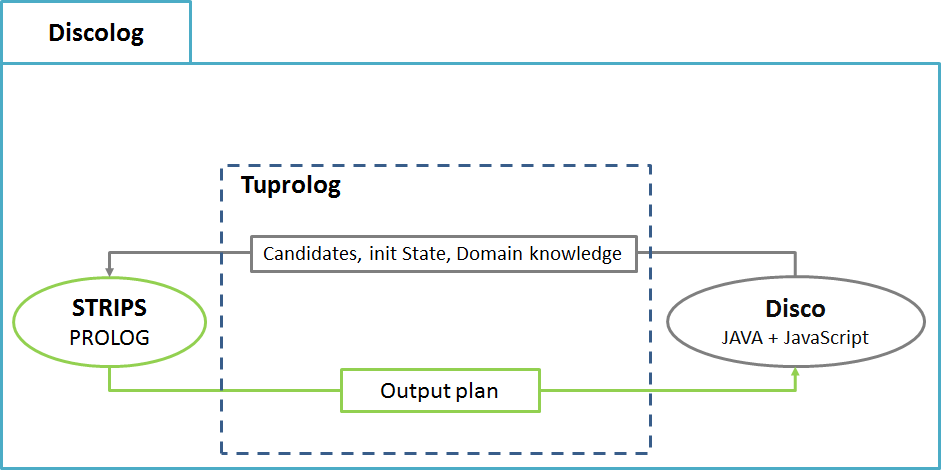
\includegraphics[width=\textwidth]{Pictures/archi1.png}
	\caption{\label{implementation environment of Discolog} implementation environment of Discolog}
\end{figure}


\section{Disco}
Disco \cite{rich2009building}is a collaborative discourse engine using reactive HTNS. The  most important feature of this reactive architecture is that allows the system to lead the user in a real time, without making any plan in advance. Disco's functional architecture is composed by a main component called \textit{task engine}. 
The function of the \textit{task engine}  is to load and validate a task model description and to maintain a representation of the current status of the user’s tasks.\cite{rich2009building}  


%----------------------------------------------------------------------------------------
\subsection{Disco task model}
Disco uses the ANSI/CEA-2018 standard for the procedural definition of the task model elements as described bellow :
\begin{itemize}
	\item \textit{Task}: The task model defines Task classes which are modeled using XML format, an example of the move\&paint implementation is showed in Appendix \ref{xml}. Primitive tasks may contain \textit{grounding script} parameter defined as JavaScript program which represent the effect of  the primitive task execution in the environment.
	
	\item \textit{Inputs and outputs} : Input includes all the data that may affect the execution of the task and output includes all data that can be affected by the execution of the task. these data type is defined in JavaScript.
	\item \textit{Conditions} : Task's conditions (Preconditions, postconditions ans applicability conditions) are defined as boolean JavaScript function to evaluate the execution of a task.

\end{itemize}

\section{Discolog implementation}
For the implementation of the Discolog system, we  faced some challenges. In addition to the management of heterogeneous environment, defining the level of information necessary to introduce in STRIPS domain knowledge required some reflection and designing a STRIPS planning algorithm able to provide effective solutions based on incomplete information in dynamic environment.
\subsection{The new Discolog API}
In order to implement the hybrid system Discolog we create an new  API divided in two mains folders :
	\begin{figure}[!h]
		\centering
		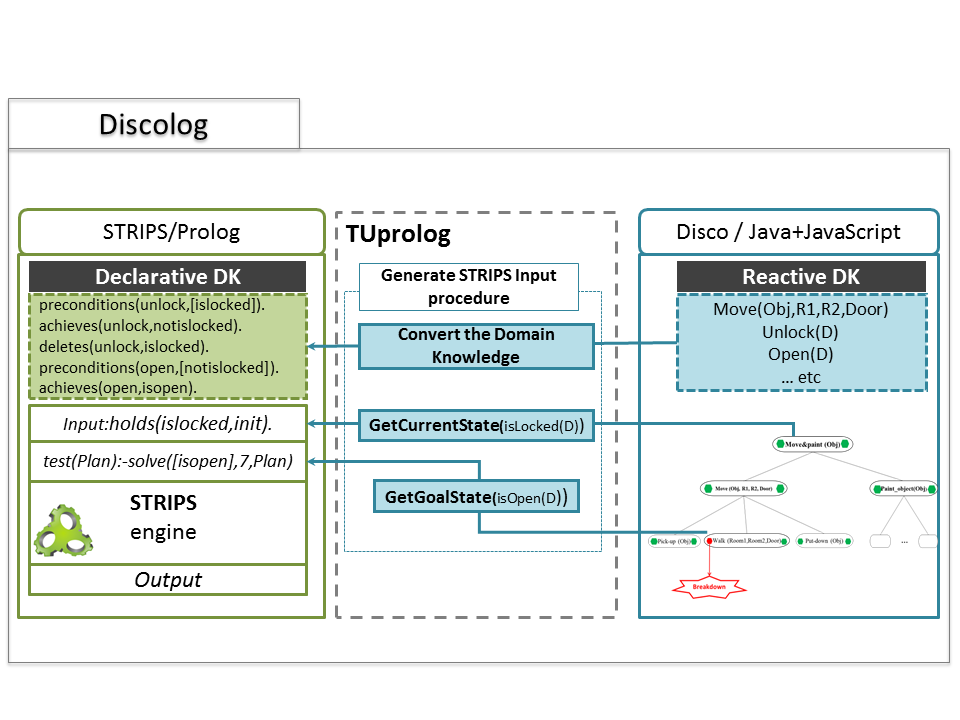
\includegraphics[width=\textwidth]{Pictures/input1.png}
		\caption{\label{input} Disco data generation in the moveandpaint example}
	\end{figure}
	
\subsubsection{ Disco extension }
We create an extension of Disco that can detect breakdowns and in such case, collects a candidates list for the plan recovery process. In addition, we manage to generate these candidates in the easiest way to be converted into Prolog formalism. The input Prolog planner is constituted in Disco via tuProlog as demonstrated in Figure \ref{input}.


 First, we start by creating the Prolog domain knowledge. Therefore, we extract all the primitives tasks and turn them to a Prolog formalism using tuProlog. Next, Disco observe the current state and convert it to the initial state. for example, in the move\&paint example, the current state where the breakdown occurs was IsLocked(Door) "the door is locked". Finally, the list of candidates is generated and each candidate is converted to a goal state to be achieve in Prolog.


\subsubsection{ Declarative Prolog implementation }
The main challenge faced in the creation of the STRIPS planner was to create an efficient means-end planning algorithm that can be integrated and executed  into tuProlog. Moreover, we had to define adequate structures that can receive the extracted domain knowledge. the STRIPS planner implemented is explained in Appendix \ref{AppendixB}.
% reference de STRIPS 


 Once STRIPS generate the plan recover, each action of this plan must be converted into primitive task formalism supported by Disco. Therefore we create a procedure that treat and convert the STRIPS plan output. An example of this procedure is shown  in Figure \ref{output} which describe how the plan repair is extracted for the move\&paint example. 

	\begin{figure}[!h]
		\centering
		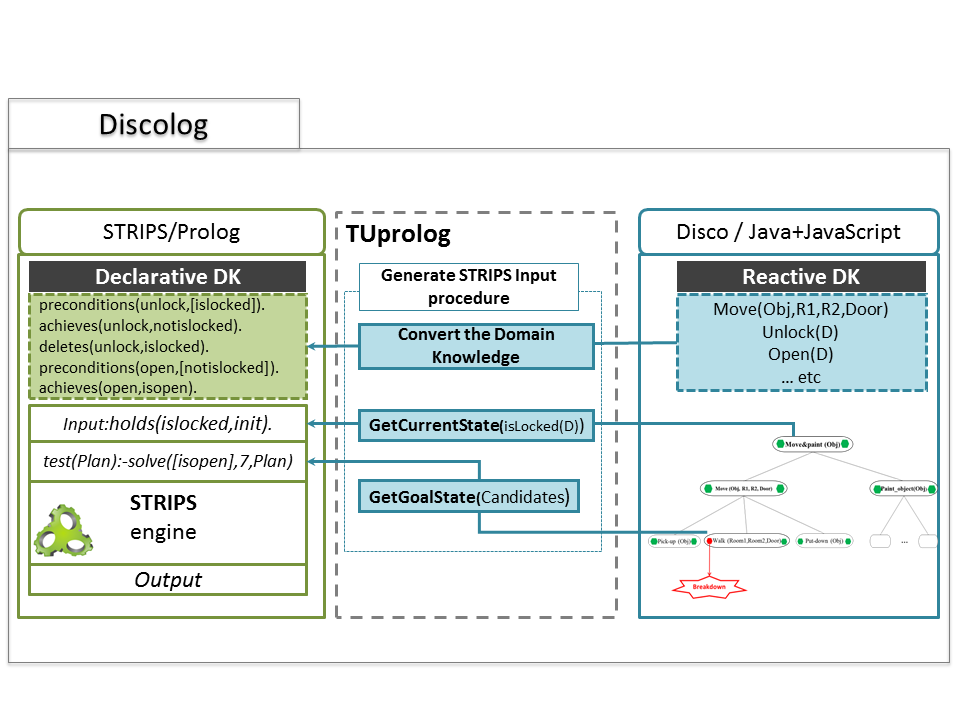
\includegraphics[width=\textwidth]{Pictures/output1.png}
		\caption{\label{output} Prolog data generation in the moveandpaint example}
	\end{figure}

\section{Conclusion}
In this chapter, we described the implementation of the Discolog system. First we introduce the environment of the implementation and we introduced the Disco system. Next we bring forward the new implemented Discolog API and explain each parts of this later.

In the next chapter, we present the experiments conducted to validate our system. 

%----------------------------------------------------------------------------------------


%\begin{multicols}{2}
%\lstinputlisting[language=XML]{Chapters/moveandpaint.xml}
%\end{multicols}
%\lstinputlisting[language=XML]{Chapters/moveandpaint.xml}
 
%\chapter{Experiments, test and results} % Main chapter title

\label{Chapter 6} % For referencing the chapter elsewhere, use \ref{Chapter1} 

\lhead{Chapter 6. \emph{Experiments, test and results}}
The experimental evaluation was devised in two mains parts, the first consisted on constructing the HTN model to evaluate the Discolog system. The second point was to variate the level of knowledge to test the robustness of  Discolog system against different types of breakdown. 
%\section{experimental environment}

\section{experimental model creation}
In order to test efficiently the Discolog system, we must test the Discolog system on different type of HTN. in the absence of accurate models. we had to create our own evaluation data. Therefore, an algorithm was constructed to generate different types of HTN models. 

The evaluation HTN was constructed using synthetic data as demonstrated in the algorithm ...
\begin{itemize}
	\item Each compound task in the HTN has a set of [$r_1$, ...,$r_\text{recipes}$].
	\item Each recipe is constituted by [$r_1$, ...,$r_\text{length}$] children to decompose the parent task.
	\item the preconditions of the first child are the same as its parent, and the postconditions of the last child are the same as its parent. 
	\item Conditions defined in the primitive tasks are chained in each recipe. Example: the task a is decomposed to \{$a_1$, $a_2$, $a_3$\}using the recipe R1. Thus, the preconditions of $a_1$ are the same as its parent a and the postconditions of $a_3$ are the same as its parent a. We define the postcondition of $a_1$ as "P1" then the preconditions of the next task $a_2$ are "P1", we also define the postconditions of $a_2$ as "P2" then the preconditions of $a_3$ task are "P2".
	\item each recipe has its applicability condition, therefore, we generated primitives tasks whose postconditions turns to true the applicability condition of each recipe, in order to be able to recover from a breakdown caused by an applicability condition failure. 
\end{itemize}
\begin{algorithm}
\caption{DiscoLog algorithm }\label{tree}
\begin{algorithmic}[]
	\Procedure{CreateHTN}{depth,length,recipes,top}
	\State $\textit{ConstructHTNTree(depth,length,recipes,top)} $

	\State $\textit{DefineLevelOfKnwoledge(top, level)} $
	\EndProcedure \textbf{EndProcedure}
	\State
	\State
	
	\Procedure{ConstructHTNTree}{depth,length,recipes,top}
	\If {$\textit{depth} > 1 $}
\For{$ \textbf{each r} \in \text{ recipes} $}
\State $\text{addRecipe(r, top)}$
\For{$ \textbf{each l} \in \text{ length} $}
\State $\text{addchild(top,childl})$
\State $ConstructHTNTree(depth,length,recipes,childl)$
\EndFor
\EndFor
\EndIf
	\EndProcedure \textbf{EndProcedure}
\end{algorithmic}
\end{algorithm}
\subsection{Test algorithm}
The Discolog system was tested on each generated model several times, and for each model, we variate the type of breakdown to recover from and the level of knowledge used in the model. We calculate the percentage of recover relative to the level of knowledge. The generated algorithm is described bellow.
\begin{algorithm}
	\caption{Test algorithm }\label{test}
	\begin{algorithmic}[]
		\Loop \text{ (10) }
\Loop (\text{Random breakdowns } $\gets$ 100)
\State(Discolog(HTN,Goal))

\EndLoop\textbf{EndLoop} \\
\EndLoop\textbf{EndLoop} \\
	\end{algorithmic}
\end{algorithm}
 
\section{ results of the Experiments} 
%\chapter[Complémentarité Vs Similarité]{Complémentarité Vs Similarité dans la relation de dominance}
\label{chap:chap6}
	\begingroup
	\parindent=0em
	\etocsettocstyle{\rule{\linewidth}{\tocrulewidth}\vskip1\baselineskip}{\rule{\linewidth}{\tocrulewidth}}
	\emph{\textbf{Sommaire}} \vspace{0.5em}
	\localtableofcontents 
	\clearpage
	\endgroup
Dans ce chapitre, nous présenterons une autre étude de l'interaction entre un utilisateur et un agent virtuel dans le contexte d'une négociation collaborative. 
Notre objectif est d'étudier l'influence de la relation interpersonnelle de dominance sur le processus de négociation. 

En premier lieu, les objectifs généraux de cette étude seront présentés (section \ref{sec:obj}). Nous détaillerons la méthodologie employée pour le paramétrage des agents utilisés dans cette expérimentation (section \ref{sec:methodo}) ainsi que les hypothèses que nous formulons (section \ref{sec:H}).

Nous présenterons ensuite le protocole expérimental employé (section \ref{sec:procedure}). Enfin, nous décrirons les résultats obtenus  (section \ref{sec:res})
que nous discuterons ensuite \ref{sec:discussion}
\section{Objectif}
\label{sec:obj}

Plusieurs études en psychologie sociale ont exploré l'impact de la relation de dominance sur l'expérience de la négociation et de ses résultats. Certains travaux ont montré que l'expression de comportements complémentaires de dominance permettait d'améliorer la coordination et donc le gain commun des négociateurs. En conséquence, les négociateurs se sentaient plus à l'aise. \cite{tiedens2003power,wiltermuth2009benefits,olekalns2013dyadic}.
En parallèle, d'autres travaux ont étudié l'impact de la similarité dans les comportements de dominance dans la négociation. Ces derniers suggèrent que la similarité dans les comportements non verbaux de dominance améliore l'interaction et le processus de négociation car les individus sont attirés par ceux qui expriment des comportements similaires. Ceci permet d'augmenter le sentiment d'affiliation \cite{olekalns2013dyadic}. 

En vue des contradictions dans la littérature sur l'impact de la complémentarité et la similarité des comportements de dominance dans les interactions, des chercheurs ont mené des études pour comparer les deux approches et étudier laquelle permettait d'avoir de meilleures influences sur l'interaction \cite{tiedens2003power,dryer1997opposites}. Ces études ont montré que la complémentarité de dominance dans les comportements non verbaux s'installait de manière inconsciente entre les individus. De plus, les participants ont préféré interagir avec les individus qui adoptaient un comportement complémentaire et se sentaient plus à l'aise comparés avec ceux qui exhibaient des comportements similaires. 


Partant de ces études, notre objectif est d'explorer l'impact de ces comportements de dominance qu'ils soient complémentaires ou similaires sur les stratégies de négociation dans le contexte d'une négociation collaborative entre un agent et un utilisateur. Cependant, comme la relation de dominance qui s'installe durant l'interaction est forcément complémentaire nous pensons que les stratégies complémentaires auront un impact positif plus important que des stratégies similaires.

\subsection{Complémentarité en psychologie sociale}
	Nous avons présenté dans la section \ref{sec:compEtat} la littérature sur les comportements complémentaires de dominance dans la négociation. Nous rappelons dans cette sections les principaux résultats: 
	
	\begin{itemize}
		\item La complémentarité dans les comportements de dominance améliore la coordination entre les négociateurs qui a pour résultat d'améliore le gain commun des négociateurs.
		
		\item La création de valeurs durant la négociation est plus importante dans des dyades où les négociateurs affichent des comportements complémentaires de dominance
		
		\item En conséquence, le sentiment de confort est accru dans les dyades complémentaires comparées aux dyades similaires. De plus, la complémentarité permet d'améliorer l'appréciation entre les négociateurs.
	\end{itemize}
	

Nous présentons dans la suite de ce chapitre notre étude qui vise à analyser ces comportements dans le contexte d'une négociation entre un agent et un utilisateur humain.

\section{Méthodologie}
\label{sec:methodo}

Afin d'illustrer notre modèle de négociation, nous reprenons le scénario d'une négociation collaborative pour le choix d'un restaurant.
Ce scénario ne nécessite aucune une expertise pour prendre part dans la négociation. De plus, il est facile pour les participants de reporter leurs préférences pour les différents critères pris en compte pour le choix d'un restaurant. En effet, nous considérons le même sujet de négociation des restaurant avec les mêmes critères. Nous avons enrichis le domaine de valeurs des critères. Chaque critère est défini avec un ensemble de valeurs présenté dans la table \ref{tab:valeursCritere}. Un total de 630 restaurants ont été générés à partir des critères regroupant les différentes possibilités.

\begin{table}[b]
	\caption{Ensemble de valeurs possible pour chaque critère afin de choisir un restaurant}
	\label{tab:valeursCritere}
	\centering
	\begin{tabular}{ >{\centering\arraybackslash}m{2cm}| >{\centering\arraybackslash}m{9cm}}
		\hline
		\hline
		\textbf{Critère} & \textbf{Ensemble des valeurs} \\
		\hline
		Cuisine & Chinois ,Français ,Italien ,Japonais ,Coréen ,Mexicain ,Turc \\
		\hline
		Ambiance & cosy ,familial ,anime ,moderne ,romantique ,calme \\
		\hline 
		Prix  & abordable ,bas prix ,chic \\
		\hline
		Localisation & centre de paris ,Gare du nord , Montparnasse , près de la tour Eiffel ,Père lachaise \\
		\hline
		\hline
	\end{tabular}
\end{table}

Trois paramètres importants sont à prendre en compte pour initialiser les comportements des agents. 
En premier lieu, il faut fixer la valeur initiale de dominance affectée à chaque agent. Nous avons choisi une valeur de dominance $dom =0.55$ afin de générer des comportements de dominance initialement neutres.

En second lieu, il faut initialiser les préférences des agents. Afin de placer les sujets dans des conditions comparables quelles que soient leurs préférences, nous avons demandé aux participants de saisir leurs préférences (voir section \ref{sec:procedure}).

A partir des préférences saisies par le participant, nous générons automatiquement les préférences des agents suivant certaines conditions.
La première condition visait à générer des modèles de préférences différents de celui communiqué par l'utilisateur dans le but de créer une confrontation qui pousse à la négociation. Pour cela, nous avons utilisé la distance de kendall \cite{bra2013Kendall}  (\emph{Kendall's  $ \tau \in [0,1]$}) afin de définir la limite minimale de différence entre le modèle de l'agent et celui de l'utilisateur. Par conséquent, nous avons fixé la distance à (\emph{Kendall's  $ \tau \geq 0.7$}).

La seconde condition assurait la différence entre les modèles de préférences générées pour les différents agents qui vont interagir avec les sujets. 
Notre objectif est d'éviter une forte ressemblance entre les préférences des agents qui donnerait l'impression d'interagir avec la même entité.

Nous avons donc gardé uniquement des modèles différents (Kendall's  $ \tau \geq 0.35$). De plus, nous avons ajouté une condition qui assure une différence de perception: pour chaque critère, les modèles devaient avoir des valeurs différentes pour représenter la valeur la plus préférée de l'agent. 
Cela permet de renforcer le sentiment d'interagir avec un agent différent, la valeur préférée étant souvent la première à être proposée par l'agent. 
%Par exemple, considérons deux modèles \emph{P1, P2} générés et qui ont une distance est supérieur à $0.35$. De plus, pour le critère \textit{cuisine}, les deux modèles ont la valeur $Italien$ comme la valeur la plus satisfiable $sat_{P1}(Italien) = 1$ et $sat_{P2}(Italien) = 1$. Ces deux modèles sont automatiquement rejetés.

En dernier lieu, nous avons paramétré la stratégie comportementale des agents. Comme notre but est d'analyser l'impact de la complémentarité ou de la similarité de la dominance durant la négociation, nous avons implémenté trois stratégies distinctes reproduisant les comportements désirés. 
A partir de notre algorithme de la théorie de l'esprit présenté dans le chapitre \ref{chap:Tom}, l'agent calcule la valeur de dominance de l'utilisateur $dom_{user}$ pour chaque tour de parole exprimé par ce dernier. Suivant la valeur de dominance calculée $dom_{user}$, l'agent adopte une des stratégies suivantes:


%	Nous avons implémenté trois agents, tous initialisé avec une valeur de dominance
%	De plus, chaque agent adopte une stratégie distincte représentant une condition expérimentale pour notre étude: 

\begin{enumerate}
	\item \textit{Comportement complémentaire}: A chaque tour de parole, l'agent révise sa valeur de dominance pour qu'elle soit complémentaire à celle détéctée pour son partenaire $dom_{agent}=1-dom_{user}$.
	
	\item \textit{Comportement similaire}: L'agent va imiter les comportements de dominance exprimées par le participant $dom_{agent} = dom_{user}$.
	
	\item \textit{Comportement neutre} : L'agent ne s'adapte pas à son interlocuteur et suit un comportement de dominance statique.
	
	 $dom_{agent} = dom_{agent} (t=0)$
\end{enumerate}

En modifiant la valeur de dominance de l'agent à chaque tour, nous avons dû ajouter une contrainte dans son modèle décisionnel afin d'assurer une cohérence dans les comportements générés. 
En effet, la valeur de dominance est essentielle pour le calcul des satisfiabilités des valeurs et un changement de cette valeur risque de fausser l'ordre des valeurs satisfiables de l'agent.
Par exemple, à un moment $t$ de la négociation, une valeur $v$ est satisfiable, mais due à une adaptation qui cause un changement de dominance la même valeur $v$ peut devenir non satisfiable. Par conséquent, l'agent peut dire à un tour aimer une valeur et aux tours suivant refuser une proposition pour cette même valeur.

En vue de protéger des préférences et donc la cohérence des comportements de l'agent, nous avons fait le choix d'utiliser uniquement la valeur de dominance initiale $dom_{agent} = 0.55$ pour calculer la satisfiabilité des valeurs.

Nous avons donc implémenté trois agents \emph{Bob, Arthur} et \emph{Kevin}. \emph{Bob} adoptant un comportement complémentaire, \emph{Arthur} qui suit un comportement similaire à celui exprimé par son partenaire de négociation, et enfin \emph{Kevin}, un agent contrôle qui suit une seule stratégie de dominance neutre. 

\section{Hypothèses}
\label{sec:H}

Suivant les travaux de \cite{tiedens2003power,dryer1997opposites,wiltermuth2015benefits}, nous supposons que la relation de dominance établie entre l'agent et l'utilisateur a une influence sur les stratégies exprimées par les négociateurs. Elle va donc avoir une conséquence sur les résultats obtenues lors de la négociation ainsi que le niveau d'appréciation à négocier avec l'agent.
Nous faisons les hypothèses suivantes: 
\begin{itemize}
	\item [$\bullet$] \textbf{H1}: Les comportements de complémentarité et de similarité des agents virtuels sont perçus par les participants.
	\item [$\bullet$] \textbf{H2}: Les négociateurs atteignent un gain commun plus important quand les négociateurs établissent une relation de dominance complémentaire.
	\item [$\bullet$] \textbf{H3}: La négociation converge plus rapidement dans le cas où les négociateurs ont une relation de dominance complémentaire. 
	\item [$\bullet$] \textbf{H4}: Le négociateur se sent plus à l'aise avec un partenaire qui exprime un comportement complémentaire.
	\item [$\bullet$] \textbf{H5}: La complémentarité dans la relation de dominance augmente l'appréciation entre les négociateurs.
\end{itemize}



\section{Protocole expérimentale}
\label{sec:procedure}
Nous présentons dans cette section, le protocole expérimental employé, en commençant par les mesures utilisées pour questionner les participants sur leurs interactions avec les différents agents. Ensuite, nous présenterons la population de participants et enfin le protocole suivi pour chaque participant. 

\subsection{Mesures}
Après chaque interaction avec un agent, le participant était invité à remplir un questionnaire sur la perception des comportements de dominance.
Nous avons repris les trois principes de dominance (voir section \ref{chap:domer}) pour évaluer les comportements des participants et des agents. De plus, pour chaque questionnaire, nous avons insérés quelques items de manipulation afin de vérifier la concordance des réponses.  Les trois principes représentent quatre comportements de dominance, à savoir :
	\begin{itemize}
		\item \textbf{D1}: La prise en compte des préférences de l'autre dans la prise de décision. Nous avons évalué l'égocentrisme des négociateurs dans leurs stratégies de négociation. 
		\item \textbf{D2}: Le niveau de concessions exprimé durant la négociation.
		\item \textbf{D3}: Le niveau d'exigence du négociateur.
		\item \textbf{D4}: Le négociateur est leader dans la négociation.
	\end{itemize}

\subsubsection{Questionnaire en auto-attribution} Les participants ont répondu pour eux-mêmes au questionnaire des comportements de dominance dans la négociation que nous avons conçu, afin de mesurer les comportements qu'ils ont exhibé durant leur interaction. Ce questionnaire utilise une échelle de Likert à 5 points. Nous présentons ci-dessous les items de ce questionnaire. 
\begin{enumerate}
	\item J'ai été égocentrique pendant la négociation
	\item J'ai pris en compte les préférences de l'agent.
	\item J'ai été exigeant(e).
	\item J'ai maintenu ma position durant la négociation.
	\item J'ai abandonné ma position durant la négociation
	\item J'ai fait des concessions pendant la négociation.	
	\item J'ai mené la négociation.
	\item J'étais leader dans la négociation
\end{enumerate}

\subsubsection{Questionnaire en hétéro-attribution}
Les participants ont répondu à un questionnaire afin de décrire leur perception de l’agent avec lequel ils interagissaient.

Nous nous sommes principalement intéressés aux comportements de dominance exprimée par l'agent. Pour cela, nous avons utilisé le même questionnaire sur les comportements de dominance (voir section \ref{sec:questionnaire})

\subsection{Questionnaire concernant l'interaction}
Pour évaluer l'appréciation du participant vis à vis de l'interaction qu'il a eu avec l'agent. Nous nous sommes basés sur les travaux de \cite{tiedens2003power,wiltermuth2009benefits,olekalns2013dyadic} pour définir le questionnaire ci-dessous:

\begin{enumerate}
	\item Je suis satisfait de la décision finale.
	\item La décision finale était équitable pour nous deux.
	\item Je me suis senti à l'aise pendant la négociation.
	\item J'ai trouvé que la négociation avec l'agent était aisée.
	\item Je me sentais détendu pendant la négociation.
	\item Je me sentais anxieux pendant la négociation.
	\item J'ai apprécié la négociation avec l'agent.
\end{enumerate}

\subsection{Données d'interactions}
Nous avons enregistré les informations suivantes à chaque interaction
\begin{itemize}
	\item Les préférences du participant et celles de l'agent.
	\item Le nombre de tours de négociation avant de trouver un compromis
	\item La position du participant dans le spectre de dominance calculé à partir de l'algorithme de théorie de l'esprit après chaque tour de parole.
	\item Le dialogue généré.
	
\end{itemize}


\subsection{Protocole}
Après avoir expliqué le but de l'étude qui portait sur l'évaluation des comportements d'agents virtuels, l'expérimentateur développait le déroulé de l'étude. 
Premièrement, il expliquait que le but de l'interaction était de négocier avec chaque agent afin de trouver un restaurant où aller dîner. Il leur donnait des instructions afin de se projeter dans une situation réelle en plus de mettre l'accent sur l'aspect "collaboratif" de la négociation comme présenté dans la figure \ref{fig:instruction}.

\begin{figure}[h]
	\fbox{\begin{minipage}{.95\textwidth}
			{\ttfamily
				\textbf{Instruction:} Mettez vous dans la situation où vous allez dîner avec un ami ou un collègue pour la première fois, vous ne connaissez pas ses goûts et il ne connaît pas les vôtres. Le but est de négocier en fonction de vos préférences respectives pour de choisir un restaurant qui \underline{vous convienne à tous les deux}.
			}
		\end{minipage}}
		
		\caption{\label{fig:instruction}Explication du but de l'étude.}
	\end{figure}
	
	
	Une fois le but de l'étude expliqué, l'expérimentateur lançait la phase de tutoriel afin de familiariser le participant à l'utilisation de l'interface de communication. L'expérimentateur présentait les différents les actes de dialogues possibles pour communiquer avec l'agent. 	
	Le participant était informé que durant cette session l'agent ne répondait pas à ses actes, et que le but était uniquement de manipuler l'interface pour générer des actes. 
	
	L’expérimentateur répondait alors à d’éventuelles questions concernant la génération d'actes de dialogue ou leurs significations.
	
	Ensuite, l’expérimentateur annonçait au participant qu’il/elle allait négocier avec trois  agents virtuels différents et
	qu’après chaque négociation, il/elle devrait répondre à différents questionnaires pour évaluer son interaction avec l’agent avec lequel il/elle venait de négocier.  Avant de commencer l'expérience, le participant est invité à saisir ses préférences pour les valeurs de chaque critère (voir la figure \ref{fig:pref}).
	
	Une fois les préférences pour les différentes valeurs de critères saisies, la fenêtre avec le premier agent s'ouvrait automatiquement invitant le participant à prendre part à la négociation. 
	
	\begin{figure}[b]
		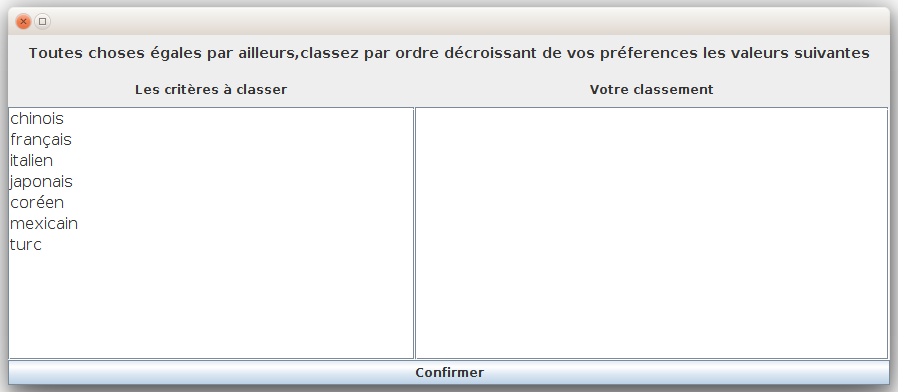
\includegraphics[width=4in]{Figures/pref.png}
		\caption{\label{fig:pref} Interface pour la saisie d'ordre de préférence. Exemple pour le critère de cuisine}
	\end{figure} 
	
	
	\subsection{Hypothèses opérationnelles}
	Nous formulons donc les hypothèses opérationnelles suivantes :
	\begin{itemize}
		\item\textit{\textbf{H1}: Les comportements de complémentarité et de similarité des agents virtuels sont perçus par les participants.}
		
			\subitem $\circ$  Les comportements de dominance attribués par les participants aux agents sont \textit{significativement différents} des comportements de dominance qu'ils se sont auto-attribués.
			\subitem $\circ$ Les comportements de dominance attribués par les participants aux agents sont \textit{similaires} aux comportements de dominance qu'ils se sont auto-attribués.
		
		\item \textit{ \textbf{H2}: Les négociateurs atteignent un gain commun plus important quand les négociateurs établissent une relation de dominance complémentaire.}
			\subitem $\circ$ Le restaurant choisi à la fin de la négociation a une valeur de satisfaction  est significativement plus importante pour les préférences des deux négociateurs dans la condition complémentaire comparé aux autres conditions. 
			
		\item [$\bullet$] \textit{\textbf{H3}: La négociation converge plus rapidement dans le cas où les négociateurs ont une relation de dominance complémentaire.}
			\subitem $\circ$ Les participants engageront plus de tours de négociations pour trouver un compromis dans la condition similaire et neutre comparé à la condition complémentaire.
		
		\item  \textit{\textbf{H4}: Le participant se sent plus à l'aise avec un partenaire qui exprime un comportement complémentaire.}
			\subitem $\circ$ Les scores de \emph{confort} perçus sont plus hauts pour l'agent complémentaire et contrôle que pour l'agent similaire.
			\subitem $\circ$ Les participants trouvent que la négociation est plus aisée avec l'agent complémentaire comparé aux autres agents.
		\item  \textit{\textbf{H5}: La complémentarité dans la relation de dominance augmente l'appréciation entre les négociateurs.}
			\subitem $\circ$ Les participants vont percevoir l'agent complémentaire comme significativement plus appréciable que l'agent similaire ou neutre.
		
	\end{itemize}
	
	\section{Résultats}
	\label{sec:res}
	Nous avons mené une étude intra-sujet dans laquelle 63 participants ont pris part. Cependant deux participants ont été écarté car ils ne remplissaient pas les conditions requises (mauvaises réponses à la majorité des questions de manipulations). Par conséquent, notre étude statistique a été mené sur les 61 participants restants. 
	
	
	%	Nous avons d'abord analyser la perception des comportements de pouvoir lors de la négociation. En effet, avant d'analyser les hypothèses, nous voudrions étudier la perception des comportements de complémentarité et la similarité durant la négociation. 
	\subsection{Perception des comportements des agents}
	

	\begin{table}[t]
		\caption{Différence de perception de dominance entre l'agent et le participant pour chaque comportement} 
		\centering
		
		\begin{tabular}{  >{\centering\arraybackslash}m{1.5cm}  >{\centering\arraybackslash}m{2.2cm}  >{\centering\arraybackslash}m{1.5cm}  >{\centering\arraybackslash}m{1.5cm}  >{\centering\arraybackslash}m{1.5cm}  >{\centering\arraybackslash}m{1.5cm}  >{\centering\arraybackslash}m{1.5cm}}
			\hline\hline
			\textbf{Agent}& Évaluation & \textbf{D1} & \textbf{D2} & \textbf{D3} & \textbf{D4} \\ 
			\hline
			
			\multirow{3}{*} {\textbf{Comp.}}  &  Z-Wilcoxon test  & -4.61 & -5.3 & -6.28 & -0.43 \\ 	
			& p-value & 2.88E-06 & 7.31E-08 & 1.42E-10 & \textbf{0.65 }\\ 
			& Effect size & -0.29 & -0.34 & -0.4 & -0.03\\ 
			\hline
			
			\multirow{3}{*} {\textbf{Similaire}}  &  Z-Wilcoxon test  & -1.57 & -2.21 & -1.45 & -1.33\\ 	
			& p-value & 0.11 & \textbf{0.024} & 0.14 & 0.17 \\ 
			& Effect size & -0.1 & -0.14& -0.09 & -0.08 \\ 
			\hline

			\multirow{3}{*} {\textbf{Neutre}}  &  Z-Wilcoxon test  & -6.23 & -5.72 & -7.056 & -0.77\\ 	
			& p value & 2.52E-10 & 6.85E-09 & 8.19E-13 & \textbf{0.4351} \\ 
			& Effect size & -0.4 & -0.36 & -0.45 & -0.049 \\ 
			\hline \hline
			
		\end{tabular}
		
		\label{tab:domPercption}
	\end{table}
	
	Pour l'analyse des différences entre les comportements de dominance des agents et des participants, des statistiques non-paramétriques ont été utilisées car la normalité des données ne pouvait être assurée. Pour l'analyse principale, le test des rangs signés de Wilcoxon a été appliqué pour évaluer chacun des quatre comportements.
	
	\subsubsection{Perception de complémentarité}
	
	Pour chaque comportement, nous avons comparé la perception des participants de leur comportements de dominance et ceux de l'agent complémentaire avec lesquels ils ont interagi. Les statistiques descriptives sont présentées dans la figure \ref{fig:comp}. 
	
	Les résultats de l'analyse de Wilcoxon ont révélé que les participants ont perçus une différence significative entre leurs comportements et celui de l'agent comme présenté dans la table \ref{tab:domPercption}. Cette différence concerne les comportements \textbf{D1, D2} et \textbf{D3}. Cependant, aucune différence significative n'a été perçu pour le comportement de leader dans la négociation \textbf{D4}. 
	\begin{figure}[h]
		\centering
		% this is wide enough
		\subfloat [Score de perception des comportements de dominance]{
			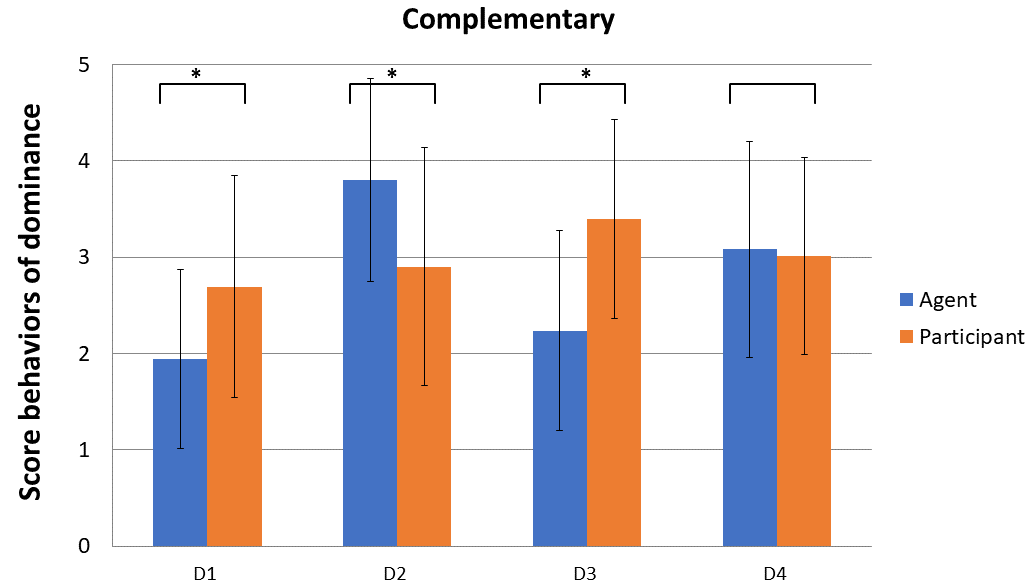
\includegraphics[clip=false]{Figures/chap7/comPow.PNG}
		}
		
		% this has a too narrow subfigure
		\subfloat[Moyenne et écart type dans les comportements de dominance]{
			\begin{tabular}{l c c c c c c}
				\hline\hline
				\textbf{Agent} & Evaluation&  \textbf{D1} & \textbf{D2} & \textbf{D3} & \textbf{D4} \\
				\hline
				
				\multirow{2}{*}{\textbf{Comp.} }& Moyenne & 1,94& 3,80 & 2,24 & 3,08 \\
				& Ecart-type & 0,93 & 1,05 & 1,03 & 1,11 \\
				
				\hline
				\multirow{2}{*}{\textbf{Part.}}& Moyenne & 2,69 & 2,94 & 3,4 & 3,02 \\
				& Ecart-type & 1,14 & 1,23 & 1,03 & 1,02\\
				\hline
				\hline
			\end{tabular}
		}
		\caption{Perception des comportements de dominance avec l'agent complémentaire}
		\label{fig:comp}
	\end{figure}	
	
	\subsubsection{Perception de similarité}
	Nous avons aussi analysé les comportements des négociateurs lors de leurs interactions avec l'agent Arthur. Les statistiques descriptives ont déjà montre une forte similarité dans la perception de tous les comportements (voir la figure \ref{fig:sim}). Nous avons complété l'étude par une comparaison de Wilcoxon a confirmé l'absence de différence significative comme présenté dans la table \ref{tab:domPercption}.  
	\begin{figure}[!tb]
		\centering
		% this is wide enough
		\subfloat[Score de perception des comportements de dominance]{
			\centering
			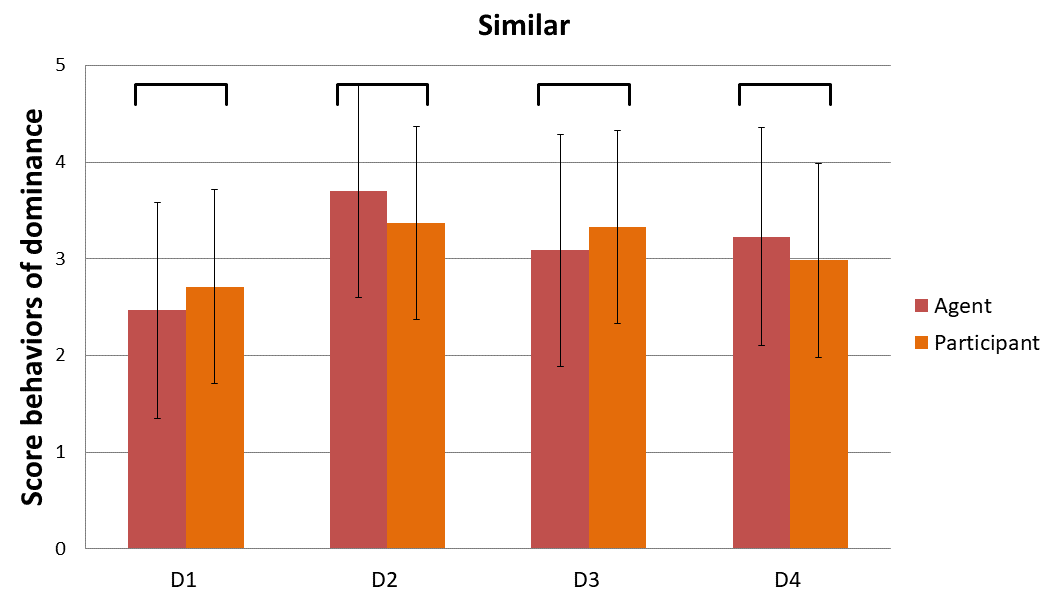
\includegraphics[clip=false]{Figures/chap7/simPow.PNG}
		}
		
		%\vspace{1em}
		% this has a too narrow subfigure
		\subfloat[Moyenne et écart type dans les comportements de dominance]{
			\centering
			\begin{tabular}{l c c c c c c}
				\hline\hline
				\textbf{Agent} & Evaluation& \textbf{D1} & \textbf{D2} & \textbf{D3} & \textbf{D4} \\
				\hline
				
				\multirow{2}{*}{\textbf{Simil.}}& Moyenne & 2,47 & 3,70 & 3,09 & 3,23 \\
				& Ecart-type & 1,11 & 1,10 & 1,19 & 1,12 \\
				
				\hline
				\multirow{2}{*}{\textbf{Part.}}& Moyenne & 2,71 & 3,37 & 3,33 & 2,98 \\
				& Ecart-type & 1,06 & 1,03 & 1,06 & 1,09\\
				\hline \hline
				
			\end{tabular}
		}
		\caption{Perception des comportements de dominance avec l'agent similaire Arthur}
		\label{fig:sim}
	\end{figure}
	
	\subsubsection{Comportement de l'agent neutre}
	
	Nous avons conduit les mêmes études statistiques pour analyser la perception des comportements de l'agent neutre. L'analyse descriptive présentée dans la figure \ref{fig:neutre} montre que les participants ont perçu que l'agent adoptait une stratégie complémentaire pour les comportements \textbf{D1}, \textbf{D2} et \textbf{D3}. Cependant, aucune différence significative n'a été perçu pour le comportement \textbf{D4}.
	
	\begin{figure}[!tb]
		\centering
		% this is wide enough
		\subfloat[Score de perception des comportements de dominance]{
			
			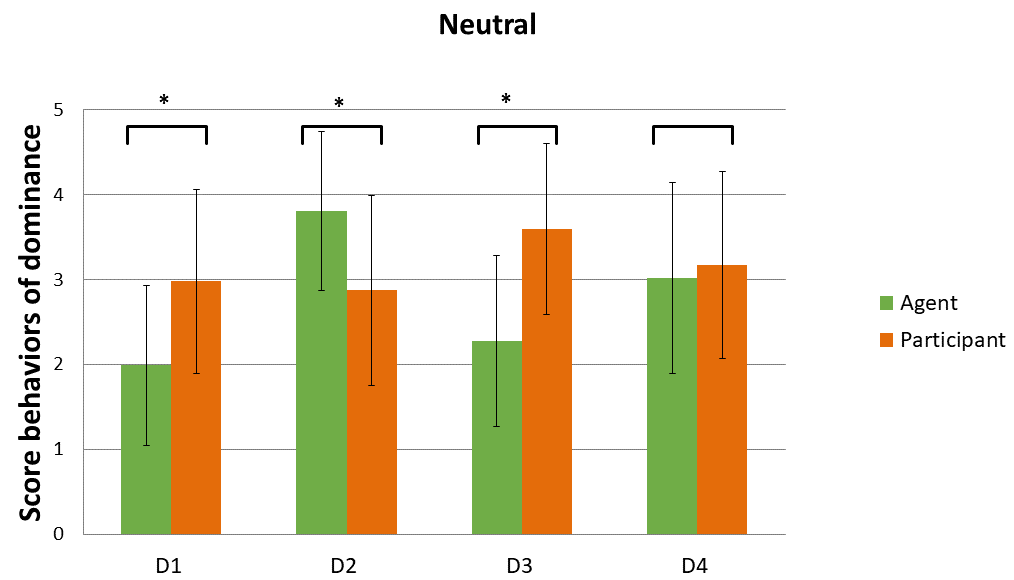
\includegraphics[clip=false]{Figures/chap7/neutrePow.PNG}
		}
		
		%\vspace{1em}
		% this has a too narrow subfigure
		\subfloat[Moyenne et écart type dans les comportements de dominance]{
			
			\begin{tabular}{l c c c c c c}
				\hline\hline
				\textbf{Agent} & Evaluation& \textbf{D1} & \textbf{D2} & \textbf{D3} & \textbf{D4} \\
				\hline
				
				\multirow{2}{*}{\textbf{Neutre}}& Moyenne & 1,99 & 3,81 & 2,28 & 3,02 \\
				& Ecart-type & 0,94 & 0,94 & 1,01 & 1,12 \\
				
				\hline
				\multirow{2}{*}{\textbf{Part}}& Moyenne & 2,98 & 2,88 & 3,60 & 3,17 \\
				
				& Ecart-type & 1,08 & 1,12 & 1,01 & 1,10 \\
				\hline \hline
				
			\end{tabular}
			
		}
		\caption{Perception des comportements de dominance avec l'agent neutre}
		\label{fig:neutre}
	\end{figure}
	
	\subsection{Gain commun}
	Nous avons analysé le gain commun des négociateurs durant les différentes négociations. Nous avons d'abord demandé aux participants leurs ressentis sur la satisfaction du restaurant choisi. Nous avons complété cette analyse par une étude objective dans laquelle nous avons calculé le score de satisfaction du restaurant choisi à partir des préférences du participant et de l'agent. L'ensemble des résultats est présenté en Annexe \ref{chap:Annexe}.
	
		\begin{figure}[h]
		
		\centering
		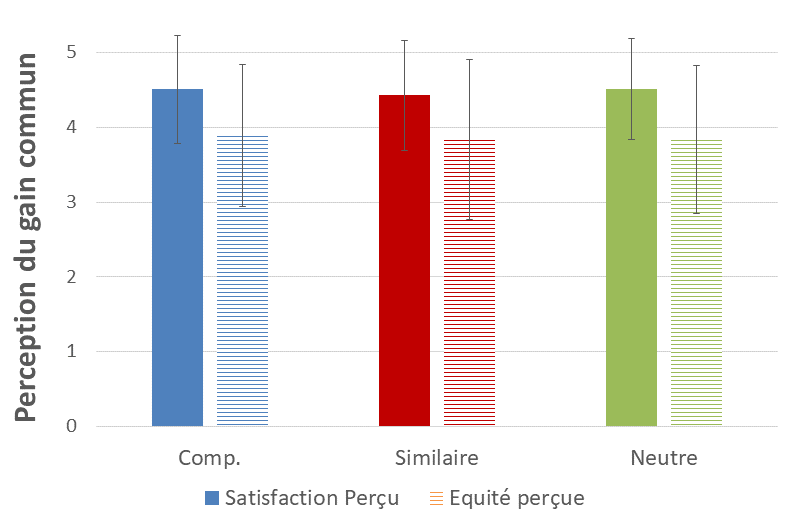
\includegraphics[width= 0.65 \linewidth,clip=false]{Figures/chap7/percpGain.PNG}
		\caption{Perception du gain commun obtenu pour tous les agents \textit{Aucune différence significative entre les agents}}
		\label{fig:gainCom}
	\end{figure}

	\subsubsection{Perception du gain commun} Nous avons demandé aux participants de renseigner leurs degrés de satisfaction du restaurant choisi avec l'agent.
	
	Les résultats sont présentés dans la figure \ref{fig:gainCom}. D'abord, les statistiques descriptives montrent qu'en moyenne les participants étaient satisfaits du restaurant choisi, et ce pour toutes les négociations. Les scores sont plutôt supérieurs à la moyenne pour tous les agents (les valeurs varient entre \emph{3.83} et \emph{4.5} sur une échelle de \emph{5}). 
	
	En outre, nous avons analysé si les participants étaient significativement plus satisfaits du restaurant choisi lors de la négociation avec l'agent Bob qu'avec les autres agents. Nous avons effectué un test de rangs signés de Wilcoxon car la normalité des données n'avait pu être assurée. L'analyse n'a montré aucune différence significative de la perception de gain et d'équité sur le choix du restaurant entre les différents agents. 
	
	\subsubsection{Analyse du gain commun } Concernant l'analyse objective du gain commun atteint à la fin de chaque négociation, nous avons dans un premier temps, récupéré les préférences des participants et des agents avec lesquels avaient interagi. 
	Ensuite, nous avons calculé la satisfiabilité du restaurant choisi pour chaque négociateur en fonction de leurs préférences (\textit{i.e. l'agent et le participant}). Nous avons ensuite, calculé le gain commun atteint à chaque négociation comme \textbf{la moyenne des valeurs de satisfiabilité} des deux négociateurs.  Les résultats obtenus pour chaque agent sont présentés dans la figure \ref{fig:gain}. 
	
		\begin{figure}[h]
		
		\subfloat[Score du gain commun atteint pour tous les agents  \textit{les populations regroupées avec $(*)$ sont significativement différentes }]{
			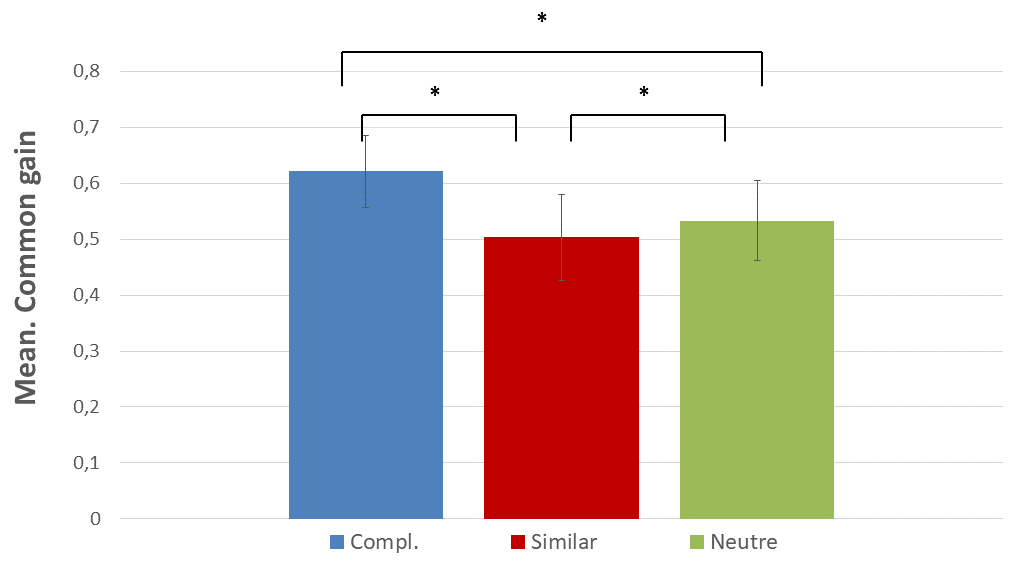
\includegraphics[clip=false]{Figures/chap7/gainCommun.PNG}}
		
		\subfloat [Score du gain commun obtenu par négociation]{
			\centering
			\begin{tabular}{l c c c}
				\hline
				\hline
				\textbf{ }& \textbf{Agent Comp.} & \textbf{Agent similaire} & \textbf{Agent neutre} \\ 
				\hline
				\newline Moyenne & 0.62& 0.5 & 0.53 \\
				\newline Écart type & 0.06 & 0.08 & 0.07 \\
				\hline
				\hline
			\end{tabular}
		}
		\caption{Les résultats obtenus pour le gain commun atteint durant la négociation}
		\label{fig:gain}
	\end{figure}

	Les valeurs de satisfiabilité sont supérieures à la moyenne pour tous les agents. Rappelons que les valeurs de satisfiabilité sont normalisées dans un intervalle $[0, 1]$. Nous avons étudié si les négociateurs avaient atteint un gain commun plus importants en négociant avec l'agent complémentaires comparés aux autres agents. En vue de la distribution normale des valeurs, nous avons appliqué un T-test afin de comparer chaque paire d'agents. Les résultats obtenus sont présentés dans la figure \ref{fig:gain}. L'analyse de la variance a montré une interaction significative entre la relation de dominance et le gain commun atteint lors des négociations. Effectivement, les participants ont atteint un gain commun significativement plus élevé en négociant avec l'agent complémentaire qu'avec l'agent similaire (\emph{t= 8.9, p < 0.01}). La même différence a été perçue en comparant avec l'agent neutre (\emph{t= 6.4, p < 0.01}).
	De plus, les participants ont atteint un meilleur gain commun avec l'agent neutre qu'avec l'agent similaire (\emph{t= 2.3, p = 0.02}).
	

	
	\subsection{Tours de paroles}
	
	Pour l'analyse de l'impact de la relation de dominance sur nombres de tours de paroles, nous avons recueilli le nombre de tours de paroles énoncé durant chaque négociation. Les statistiques descriptives sont présentées dans la figure \ref{fig:tour}. Un test paramétrique a été utilisée car les données suivent une distribution normale. Les résultats montrent que la négociation convergeait significative plus rapidement quand les participants négociaient avec l'agent complémentaire par rapport à l'agent similaire (\emph{t= 2.7, p = 0.003}). De même, la négociation convergeait plus rapidement avec l'agent neutre comparé à l'agent similaire (\emph{t= 4.43, p < 0.01}).  Les résultats sont présentés en Annexe \ref{chap:Annexe}.
	Cependant, aucune différence significative n'a été perçu entre l'agent complémentaire et l'agent neutre (\emph{t= 1.3, p = 0.09}).  
	
	\begin{figure}[!tbh]
		
		\subfloat[Nombre de tours de paroles durant une négociation pour tous les agents \textit{les populations regroupées avec $(*)$ sont significativement différentes}] {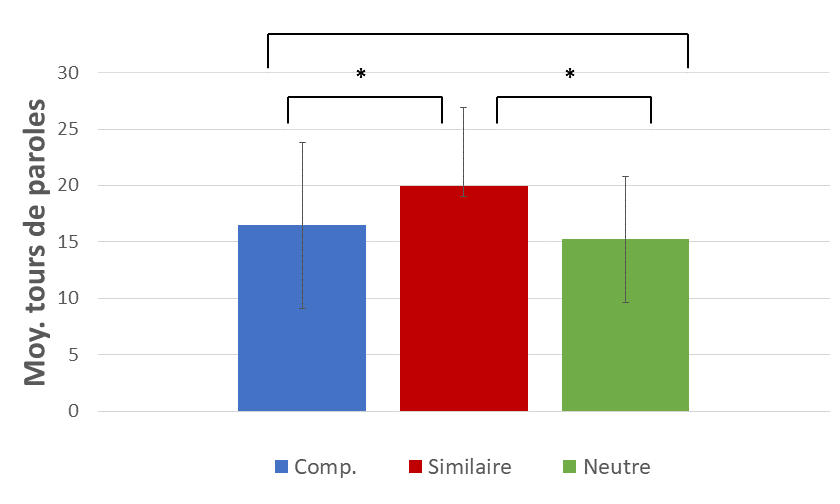
\includegraphics{Figures/chap7/tours.PNG}}
		
		
		\subfloat[Nombre de tours de paroles par négociation]{
			\centering
			\begin{tabular}{ l c c c }
				\hline
				\hline
				\textbf{ }& \textbf{Agent Comp.} & \textbf{Agent similaire} & \textbf{Agent neutre} \\ 
				\hline
				\newline Moyenne & 16.61& 19.94 & 15.13 \\
				\newline Écart type & 7.38 & 6.87 & 5.6 \\
				\hline
				\hline
			\end{tabular}
		}
		\caption{Résultats pour l'hypothèse H3.}
		\label{fig:tour}
	\end{figure}
	
	
	\subsection{Confort}
	
	Les statistiques descriptives sont présentées dans la table \ref{tab:confort}. Les participants se sont globalement sentis à l'aise avec tous les agents.
	Les score de détente ressentie sont au-dessus de 3,4 (sur une échelle à 5 points) pour tous les agents. Au contraire, les scores relatifs à l'anxiété  ressentie sont au-dessous de 2 (sur une échelle à 5 points) pour tous les agents. 
	
	Afin d'analyser une différence dans le confort perçue, nous avons utilisé un test non paramétrique car la normalité n'a pas pu être assurée. Le test de rang signé de Wilcoxon a été appliqué afin d'analyser si les participants se sont sentis plus à l'aise avec l'agent complémentaire qu'avec les autres agents. (Voir résultats en annexe \ref{chap:Annexe}). 
	Les résultats montrent que les participants se sont sentis plus à l'aise avec l'agent complémentaire qu'avec l'agent similaire (\emph{Z= -2.73, p = 0.002})
	avec un effet de taille faible (\emph{e = -0.1}). Cependant, aucune différence significative n'a été perçu entre l'agent complémentaire et l'agent neutre. 
	
	
	\begin{figure}[h]
		
		\subfloat[Score de confort que les participants ont ressenti pour tous les agents. \textit{les populations regroupées avec $(*)$ sont significativement différentes }]{
			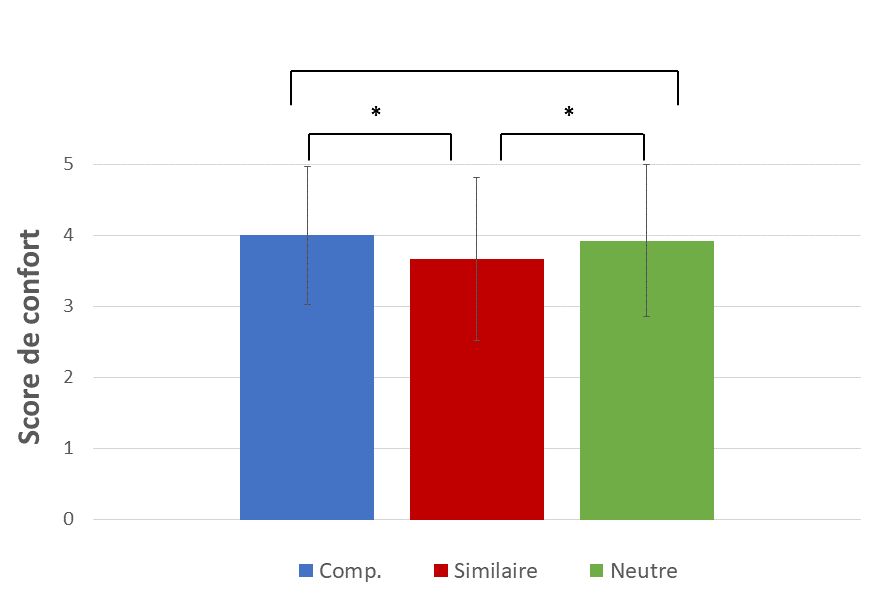
\includegraphics[clip=false]{Figures/chap7/confort.PNG}
		}
		
		\subfloat[L'effet de la relation de dominance sur le confort ressenti pendant la négociation avec l'agent]{
			\centering
			\begin{tabular}{ l l c c c  }
				\hline\hline
				\textbf{ }& & \textbf{Agent Comp.} & \textbf{Agent similaire} & \textbf{Agent neutre} \\ 
				\hline
				\newline \newline\multirow{2}{*} {Détendu} & Moy. &3.79 & 3.47 & 3.79 \\
				\newline  & SD & 1 & 1.2 & 1 \\
				\hline
				
				\newline \newline\multirow{2}{*} {Anxieux} & Moy. & 1.79 & 2.13 & 1.93 \\
				\newline  & SD & 7.38 & 6.87 & 5.6 \\
				\hline\hline
			\end{tabular}
		}
		\caption{Résultats pour la perception du confort durant la négociation.}
		\label{tab:confort}
	\end{figure}	
	\vspace{- 1 em}
	
	\subsection{Appréciation}
	Les statistiques descriptives concernant les scores d’appréciation sont présentées dans la figure \ref{fig:app}. Globalement,
	les scores sont centrés autour de 3.7 (sur une échelle de 5). L'analyse de variance montre l'effet de la relation de dominance sur la perception de l'appréciation. Les résultats sont présentés en annexe \ref{chap:Annexe}.
	
	\begin{figure}[h]
		
		\subfloat[Score d'appréciation perçue pour tous les agents. \textit{les populations regroupées avec $(*)$ sont significativement différentes}]{
			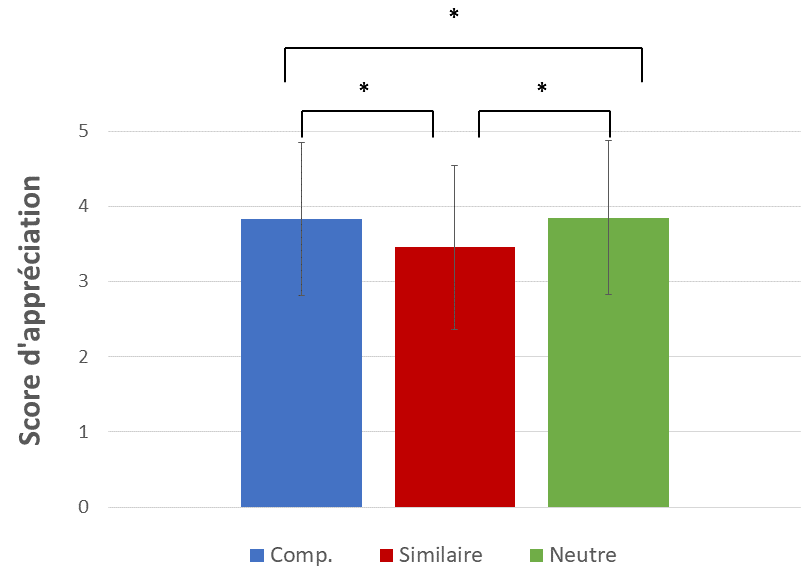
\includegraphics[clip=false]{Figures/chap7/appreciation.PNG}
		}
		
		\subfloat[L'effet de la relation de dominance sur l'appréciation perçue]{			
			
			\begin{tabular}{ l c c c c c }
				\hline\hline
				\textbf{ }& \textbf{Agent Comp.} & &  \textbf{Agent similaire} & & \textbf{Agent neutre} \\ 
				\hline
				\newline Moy. & 3.83 & &3.46 & & 3.85 \\
				\newline SD & 1.01 & & 1.09& &  1.02 \\
				\hline\hline
				
			\end{tabular}
		}
		\caption{Résultats pour la perception de l'appréciation.}
		\label{fig:app}
	\end{figure}
	
	
	Le test de rangs signé de Wilcoxon montre que l'agent complémentaire a été perçu comme significativement plus agréable que l'agent similaire (\emph{p < 0.01, Z = -3.17}). Par ailleurs, l'agent neutre a aussi été perçu comme plus agréable que l'agent similaire (\emph{p < 0.01, Z = -3.3}). Cependant, aucune différence n'a été perçu entre l'agent complémentaire et l'agent neutre (\emph{p = 0.6, Z = -0.31}).
	
	Nous nous sommes aussi intéressés à la facilité de collaboration entre le participant et l'agent. En effet, nous avons demandé aux participants de relater le degré de facilité de négociation avec l'agent. Les résultats sont présentés dans la figure \ref{fig:aise}. En général, les participants ont trouvé que la négociation été aisée avec l'agent complémentaire (\emph{M= 4, SD = 1}) ainsi qu'avec l'agent neutre (\emph{M=3.9, SD =0.99}). Les participants ont perçue la négociation avec l'agent similaire comme moins aisée (\emph{M=3.16, SD = 1.06}). 
	Nous avons ensuite analysé si cette différence de perception été significative. Comme les données ne sont pas normalement distribué, nous avons appliqué le test de rangs signé de Wilcoxon. Les résultats montrent qu'en effet les participants ont trouvé que négocier avec l'agent similaire été significativement moins aisée comparé à l'agent complémentaire (\emph{p < 0.01, Z = -3.86} avec un effet de taille moyen \emph{e = -0.35}) et l'agent neutre (\emph{p < 0.01, Z = -3.61} avec un effet de taille moyen \emph{e = -0.32}).
	Cependant, aucune différence n'a été perçue entre l'agent complémentaire et l'agent neutre.
	\begin{figure}[h]
		
		\subfloat[Évaluation de la collaboration durant la négociation. \textit{les populations regroupées avec $(*)$ sont significativement différentes }]{
			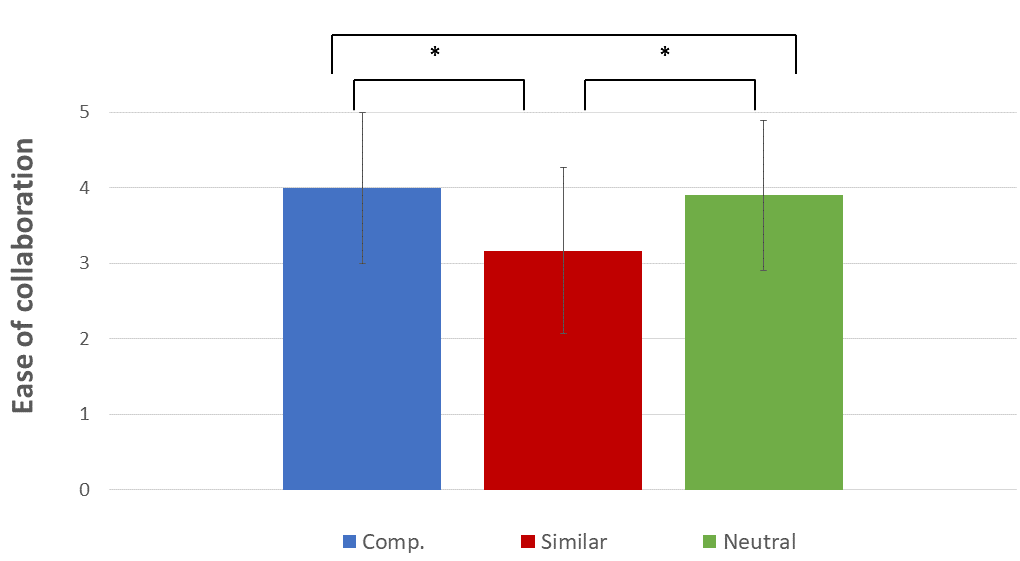
\includegraphics[clip=false]{Figures/chap7/aisee.PNG}
		}
		
		\subfloat[L'effet de la relation de dominance sur la facilité de collaboration]{
			\centering
			\begin{tabular}{ l c c c c c }
				\hline\hline
				\textbf{ }& \textbf{Agent Comp.} & &  \textbf{Agent similaire} & & \textbf{Agent neutre} \\ 
				\hline
				\newline Moy. & 4 & & 3.16 & & 3.9 \\
				\newline SD & 1 & & 1.09  & & 0.99   \\
				\hline\hline
				
			\end{tabular}
		}
		\caption{Résultats pour la facilité de collaboration durant la négociation.}
		\label{fig:aise}
	\end{figure}
	
	
	\section{Analyses complémentaires}
	Dans le chapitre 2, nous présentons la relation de dominance comme une relation interpersonnelle qui s'établie durant l'interaction. 
	Par conséquent, en plus du trais de personnalité, un individu est influencé par l'environnement de l'interaction (\textit{ex.} contexte de l'interaction, rôle social ...). Ces différents paramètres vont créer une certaine relation de dominance qui peut varier d'une interaction à une autre.  
	Afin de vérifier si les participants produisaient différents comportements de dominance durant les différentes négociations, nous avons recueilli la perception de l'agent des comportements de dominance de son interlocuteur.  Les résultats sont présentés dans la figure \ref{fig:dom}.
	
	Nous avons analysé, pour le même participant, la variance des comportements de dominance à travers les trois négociations. Pour ce faire, nous avons utilisé le test de rang signé de Wilcoxon car la normalité des données n'a pu être assurée. 
	
	Les résultats montrent les comportements de dominance des participants variaient d'une interaction à une autre. En effet, le test de Wilcoxon révèle une différence significative entre les comportements perçus par l'agent complémentaire et l'agent similaire (\emph{p<0.01, Z = -3.35}). Ces mêmes résultats sont observés en comparant la perception de l'agent complémentaire et l'agent neutre (\emph{p< 0.01, Z = -3.88}).
	Toutefois, aucune différence entre l'agent similaire et l'agent neutre n'a été vérifié (\emph{p = 0.6, Z = 0.44}). 
	
	Ces résultats suggèrent que les participants ont adopté une stratégie de négociation différente en fonction de la relation établie avec l'agent. 
	
	\begin{figure}[h]
		
		\subfloat[Évaluation de comportements de dominance des participants perçus par les agents. \textit{les populations regroupées avec $(*)$ sont significativement différentes }]{
			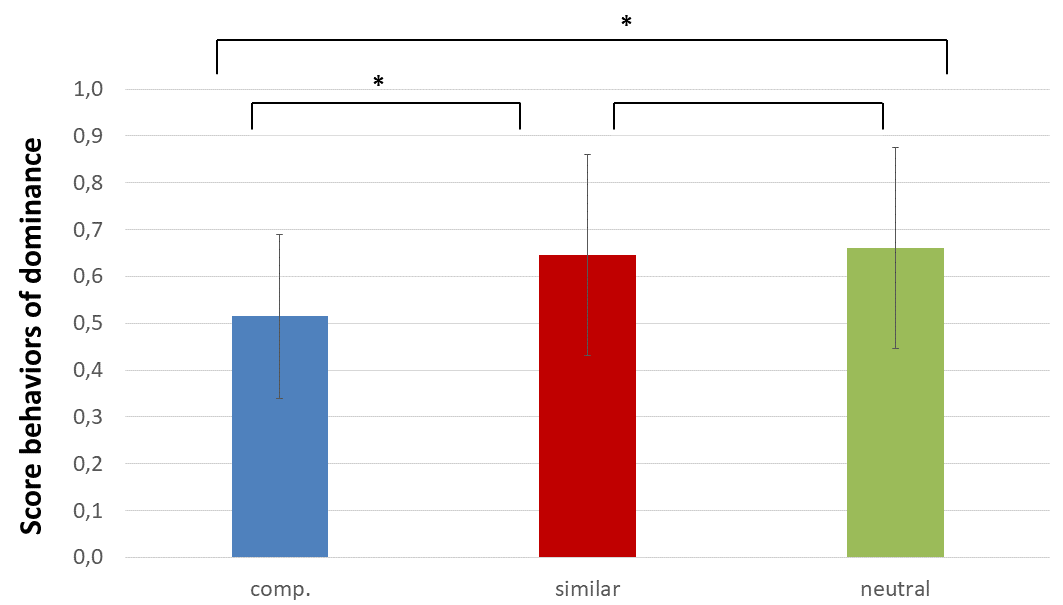
\includegraphics[clip=false]{Figures/chap7/pow.png}
		}
		
		\subfloat[Perception de l'agent des comportements de dominance exprimés par les participants]{
			\begin{tabular}{ l c c c c c }
				\hline
				\hline
				\textbf{ }& \textbf{Agent Comp.} & &  \textbf{Agent similaire} & & \textbf{Agent neutre} \\ 
				\hline
				\newline Moy. & 0.51 && 0.64 && 0.66 \\
				\newline SD & 0.17 && 0.21 && 0.219   \\
				\hline
				\hline
			\end{tabular}
		}
		\caption{Résultats pour la variation des comportements de dominance à travers les interactions.}
		\label{fig:dom}
	\end{figure}
	
	\section{Discussion}
	\label{sec:discussion}
	En général, toutes nos hypothèses ont été validées. Ces résultats appuient la validité de notre modèle négociation collaborative et de théorie de l'esprit dans le cadre d'une interaction agent/humain.   
	
	\subsection{Perception des comportements des agents}
	Notre hypothèse H1 (\textit{les comportements de complémentarité et de similarité des agents virtuels sont perçus par les participants}) est partiellement validée. 
	
	Quatre comportements de dominance ont été pris en compte pour mesurer la stratégie de négociation. 
	Les participants ont été en mesure de distinguer une différence significative de trois comportements sur quatre entre leurs stratégies et celle de l'agent complémentaire.
	
	En effet, les participants ont perçu une différence entre leurs niveaux d'exigences et de concessions \textbf{D3}, \textbf{D2}, ainsi que la prise en compte des préférences de l'autre \textbf{D1}. Cependant, aucune différence n'a été perçu concernant les comportements de leadership durant la négociation \textbf{D4}. 
	
	Concernant, les comportements de l'agent neutre, ce dernier a été perçu comme significativement complémentaires aux utilisateurs pour les comportements \textbf{D1}, \textbf{D2} et \textbf{D3}. 
	Toutefois, comme l'agent complémentaire, aucune différence n'a été perçue dans les comportements relatifs à \textbf{D4} entre l'agent neutre et les participants. 
	
	Nous avons étudié les données afin de comprendre pourquoi les participants ne percevaient pas de différence dans les comportements de leadership. 
	
	Concernant l'agent complémentaire, les comportements de leaderships ont pu être masqué à cause de  sa stratégie d'adaptation qui modifié ses comportements de dominance à chaque tour de parole.
	
	En outre, l'aspect collaboratif de la négociation pourrait avoir atténué la perception du leadership dans la négociation ce qui pourrait expliquer le cas de l'agent neutre. 
	
	Enfin, l'absence de résultats pour les deux agents nous amènent à nous questionner sur les items proposés pour mesurer le leadership. 
	Il serait intéressant de faire une évaluation post-hoc afin de demander aux participants le types de comportements qu'identifieraient le leadership durant la négociation.
	
	En parallèle, les participants ont perçu une similarité entre leurs comportements et ceux de l'agent similaire. En moyenne, pour chaque comportement, les valeurs assignés en auto-attribution et en hétéro sont très proches. De plus, l'absence de différence significative appuie ce résultat. Nous sommes conscients que l'absence de différence n'est pas une assurance de similarité de perception. Cependant, il est difficile de trouver un calcul statistique qui assure la similarité entre deux populations.
	
	D’un point de vue plus général, les résultats obtenus appuient la cohérence de notre modèle de décision tant sur la perception des comportements de dominance que sur la capacité de l'agent à percevoir les comportements de son interlocuteur et de s'y adapter correctement.  
	
	Par ailleurs, la perception des comportements de l'agent neutre comme complémentaires à ceux des participants soutient que la relation interpersonnelle de dominance qui s'établie au cours de l'interaction est complémentaire \cite{burgoonnonverbal}. En effet, indépendamment des deux autres agents où nous avions manipulé l'adaptation de l'agent, dans la condition neutre l'agent ne s'adapte pas aux comportements du participant. Néanmoins, les résultats démontrent que le participant s'est adapté aux comportements exhibés par l'agent et a ainsi établie une relation interpersonnelle de dominance complémentaire.
	
	\subsection{Gain commun}
	Notre seconde hypothèse (\textit{Les négociateurs atteignent un gain commun plus important quand les négociateurs établissent une relation de dominance complémentaire.}) est validée. 
	
	Nous avons en premier temps demandé aux participants de relater leur avis sur le restaurant choisi pour chaque négociation.
	En général, les participants ont été satisfaits du choix final et le trouvaient équitable pour toutes les négociations. 
	En analysant la valeur de satisfiabilité du restaurant choisi pour les préférences des participants (voir table \ref{tab:gainPerceptif}), les valeurs étaient autour de 0.7 (\emph{min =0.69, max = 0.73}). 
	
	Cependant, en analysant la valeur de satisfiabilité pour les préférences de l'agent,  en moyenne, seul l'agent complémentaire a pu converger vers un restaurant qui respecte ses préférences (\emph{M = 0.53, SD = 0.2}). 
	
	
	\begin{table}
		\centering
		\caption{Moyenne des valeurs de satisfiabilité du restaurant choisi pour chaque négociateur} 
		\begin{tabular} {lcccccccc}
			\hline
			\hline
			& \multicolumn{2}{c}{Agent Comp.} & & \multicolumn{2}{c}{Agent similaire}& & \multicolumn{2}{c}{Agent neutre} \\ % column 4 blank, for spacing
			\cline{2-3} \cline{5-6} \cline{8-9} % horizontal lines connecting cols. 2-3, 5-6
			& Part. & Agent & & Part. & Agent & &  Part. &Agent \\ \hline
			Moy. &0,71 & 0,53 & &  0,69 & 0,33 & & 0,73 & 0,34 \\
			SD & 0,2 & 0,24 & &  0,18 & 0,19 & & 0,18 & 0,16 \\
			\hline
			\hline
		\end{tabular}
		\label{tab:gainPerceptif}
		
	\end{table}
	
	Concernant l'agent similaire, la moyenne de satisfiabilité est assez basse. Ceci est causé par le fait que les négociateurs ne communiquaient pas bien durant la négociation. Par conséquent, la négociation durait plus longtemps causant la chute de la courbe de concession $Self$. De ce fait, l'agent faisait plus de concession et finissait par accepter un restaurant dont la satisfiabilité n'était pas élevée (\emph{M = 0.33, SD = 0.18}).
	
	Concernant l'agent neutre qui n'est pas très dominant, il est normal que dans la majorité des cas, la courbe de concession finissait par décroitre menant l'agent à faire des concessions importantes. Ceci explique la moyenne de satisfiabilité atteinte par l'agent neutre  (\emph{M = 0.34, SD = 0.16}).
	
	Cette analyse confirme les résultats de l'étude objective menée.
	Pour toutes les négociations, nous avons comparé le gain commun et nous avons observé qu'il était significativement plus important durant les négociations avec l'agent complémentaire comparé aux autres agents. De plus, les négociateurs avaient de meilleurs gains durant la négociation avec l'agent neutre comparé à l'agent similaire. Ceci prouve que la relation complémentaire qui s'est installé durant la négociation avec l'agent neutre a permis un meilleur échange d'information. 
	
	Ces résultats confirme que les négociateurs communiquent mieux et par conséquent négocient mieux dans le cadre d'une relation complémentaire de dominance.  
	
	
	\subsection{Tours de paroles}
	Notre hypothèse H3 (\textit{La négociation converge plus rapidement dans le cas où les négociateurs ont une relation de dominance complémentaire}) est validée. En effet, la négociation convergeait en moyenne plus rapidement quand une relation de dominance complémentaire s'établissait entre l'agent et le participant. De plus, dans cette même condition le gain commun atteint par les négociateurs était plus important. Ainsi, ces résultats appuient les théories de  psychologie sociales selon lesquelles la relation interpersonnelle de dominance améliore la coordination et l'échange d'informations.
	
		
	En ce qui concerne l'agent neutre, la négociation convergeait rapidement à cause de deux raisons. Premièrement, avec une valeur de dominance initialisée à 0.5, l'agent avait un niveau d'exigence moyen ce qui facilitait le processus pour trouver un compromis. 
	Deuxièmement, d'après nos résultats, dans cette condition, une relation complémentaire de dominance s'était établie entre les négociateurs ce qui facilitait la coordination. 
	
	En conclusion, la relation interpersonnelle de dominance améliore la coordination et l'échange d'information qui résulte en des processus de négociation court et plus efficaces. 
	
	\subsection{Appréciation de l'agent}
	Nos hypothèses H4 (\textit{Le négociateur se sent plus à l'aise avec un partenaire qui exprime un comportement complémentaire})  et H5  (\textit{La complémentarité dans la relation de dominance augmente l'appréciation entre les négociateurs.}) sont validées. 
	
	Pour l’appréciation, les scores sont au-dessus de la moyenne pour tous les agents. Ce pourrait être le reflet d’un léger biais positif envers les agents. Toutefois, l'analyse des différences a révélé que les participants ont significativement plus apprécié la négociation avec l'agent complémentaire que l'agent similaire. De même, les participants ont jugé que l'agent neutre était aussi plus agréable que l'agent similaire. 
	
	En outre, nous avons analysé le confort ressenti lors de la négociation. Globalement, les participants se sont sentis détendus durant la négociation et ont trouvé la négociation confortable avec tous les agents.  
	
	L'analyse de variance a révélé que les participants se sont plus sentis à l'aise avec l'agent complémentaire qu'avec l'agent similaire. Cependant, aucune différence n'a été perçu entre l'agent complémentaire et l'agent neutre, et entre l'agent neutre et l'agent similaire.
	
	En plus du confort, nous avons analysé la facilité de collaborer avec l'agent durant la négociation. Les résultats montent que les participants ont perçu le processus de négociation comme plus aisé avec l'agent complémentaire et l'agent neutre qu'avec l'agent adoptant une stratégie similaire à la leurs. 
	
	Ces résultats confirment nos hypothèses. Les participants préfèrent négocier avec un partenaire avec lequel ils ont établi une relation complémentaire qu'avec un négociateur qui exhibe des comportements de dominance similaires. 
	
	
	\section{Conclusion}
	Pour cette quatrième étude, nous avions pour objectif d'étudier l'effet de la relation de dominance sur la négociation entre un agent et un participant humain. Nous nous sommes basés sur les travaux de Tienders et Wiltermuth \cite{wiltermuth2009benefits,tiedens2003power} qui affirment que la complémentarité dans la relation de dominance avait un impact positif sur la négociation. 
	
	Nous avons implémenté trois agents négociateurs adoptant trois stratégies différentes, un agent complémentaire, un agent similaire et un agent neutre. 
	63 participants ont pris part à  des négociations collaboratives avec ces agents dans le but de trouver un restaurant qui satisfassent leurs préférences. 
	
	Les résultats ont confirmé la majorité de nos hypothèses et nous ont permis d'aller plus loin dans l'analyse des comportements de dominance dans la négociation. 
	
	D'abord, nous avons pu valider notre modèle de la théorie de l'esprit dans le cadre d'une interaction avec un utilisateur humain. 
	Les résultats montrent que les participants ont été capables de percevoir une différence dans les stratégies qu'adoptaient les agents. Ceci nous permet de valider la robustesse des prédictions de notre modèle. 
	
	Par ailleurs, toutes les hypothèses relatives à l'effet positif de la relation de dominance complémentaire ont été validées. Quand les négociateurs établissaient une relation de dominance complémentaire, ils atteignaient un meilleur gain commun et ceux dans un délai plus court comparés aux autres configurations. La négociation était vécue comme plus agréable et confortable et les négociateurs semblaient mieux collaborer. 
	
	Les résultats ont aussi révélé des comportements qui soutiennent les travaux en psychologie sociale. En effet, en analysant les comportements exprimés lors des négociations avec l'agent neutre, nous nous sommes rendu compte qu'une relation complémentaire de dominance s'était installé entre les négociateurs. Ces résultats appuient la définition de Dunbar and Burgoon \cite{dunbar2005perceptions} qui affirment que la relation de dominance est forcément complémentaire. En outre, la relation de dominance étant interpersonnelle, elle s'établie durant l'interaction. Ce point a aussi été validé par nos analyses qui nous ont permis de montrer que les participants ont adopté des comportements de dominance différents d'une négociation à une autre. Cela suggère que les négociateurs s'adaptent à leur interlocuteur pour définir une relation de dominance propre à l'interaction.  

%----------------------------------------------------------------------------------------
%	THESIS CONTENT - APPENDICES
%----------------------------------------------------------------------------------------

\addtocontents{toc}{\vspace{2em}} % Add a gap in the Contents, for aesthetics

\appendix % Cue to tell LaTeX that the following 'chapters' are Appendices

% Include the appendices of the thesis as separate files from the Appendices folder
% Uncomment the lines as you write the Appendices

%% Appendix A

\chapter{Move\&paint task in Disco} % Main appendix title

\label{xml} % For referencing this appendix elsewhere, use \ref{AppendixA}

\lhead{Appendix A. \emph{Move\&paint task in Disco}} % This is for the header on each page - perhaps a shortened title
\begin{verbatim}
<taskModel about="urn:limsi.fr:examples:moveandpaint
"xmlns="http://ce.org/cea-2018">

<task id="move_paint">
<input name="box" type="Box"/>
<subtasks id="movepaint">
<step name="move" task="move"/>
<step name="paint" task="paint"/>
<binding slot="$move.box" value="$this.box"/>
<binding slot="$move.from" value="$this.box.location"/>
<binding slot="$move.to" value="Room.ENUM.Painting_Room"/>
<binding slot="$paint.box" value="$move.new_box"/>
</subtasks>
</task>

<task id="move">
<input name="box" type="Box" modified="new_box"/>
<input name="from" type="Room"/>
<input name="to" type="Room"/>
<output name="new_box" type="Box"/>

<subtasks id="move_id">
<step name="pickup" task="pickup"/>
<step name="walk" task="walk"/>
<step name="putdown" task="putdown"/>
<binding slot="$pickup.box" value="$this.box"/>
<binding slot="$walk.box" value="$this.box"/>
<binding slot="$walk.from" value="$this.from"/>
<binding slot="$walk.to" value="$this.to"/>
<binding slot="$putdown.box" value="$walk.new_box"/>
<binding slot="$this.new_box" value="$walk.new_box"/>

</subtasks>
</task>

<task id="pickup">
<input name="box" type="Box"/>
</task>  

<task id="walk">
<input name="box" type="Box" modified ="new_box"/>
<input name="from" type="Room"/>
<input name="to" type="Room"/>
<output name="new_box" type="Box"/>

<precondition> isOpen() </precondition> 
<postcondition sufficient="true">
 $this.new_box.location == $this.to
 </postcondition> 
<script>$this.new_box.location = $this.to;</script>
</task>

<task id="putdown">
<input name="box" type="Box"/>
</task>

<task id="paint">
<input name="box" type="Box" modified ="new_box"/>
<output name="new_box" type="Box"/>
<precondition> 
$this.box.location == Room.ENUM.Painting_Room
 </precondition>
<postcondition sufficient="true"> $this.new_box.paint </postcondition>
<script> $this.new_box.paint = true; FIRST_PAINT = false; </script>
</task>

<task id="open">
<precondition> !isLocked(); </precondition>
<script> OPEN = true; </script>
</task>

<task id="unlock">
<script> LOCKED = false; </script>
</task>
<task id="recovery"/>  
<script init="true">

function Box (name,location, paint) {
this.name = name;
this.location = location;
this.paint = paint;
}

Box.prototype.toString = function () { 
return (this.name+ "[" + this.location+ "," + this.paint+"]");}

function Room (name) { 
this.name = name; 
}

Room.ENUM = { Room1 : new Room("room1"), 
Painting_Room : new Room("painting_room"),
 }
Room.prototype.toString = function ()
{ return this.name;}

var BOX1 = new Box("box1", Room.ENUM.Room1, false);
var OPEN = true;
var LOCKED = false;
var FIRST_PAINT = true;
var LOCATION = Room.ENUM.Room1; 
function isOpen() { return OPEN; }
function isLocked() { return LOCKED; }

</script>  
</taskModel>
\end{verbatim}
%\input{Appendices/AppendixB}
%\input{Appendices/AppendixC}

%\addtocontents{toc}{\vspace{2em}} % Add a gap in the Contents, for aesthetics
%
%\backmatter
%
%%----------------------------------------------------------------------------------------
%%	BIBLIOGRAPHY
%%----------------------------------------------------------------------------------------
%
\label{Bibliography}
%
\lhead{\emph{Bibliography}} % Change the page header to say "Bibliography"
%
%\bibliographystyle{unsrtnat} % Use the "unsrtnat" BibTeX style for formatting the Bibliography
%
\bibliography{Bibliography} % The references (bibliography) information are stored in the file named "Bibliography.bib"
\bibliographystyle{plain}
%
%\bibliography{Bibliography}
\end{document}  